
\section{Experimental evaluation}
\label{sec:ncdn-eval}


We conduct trace-driven experiments to compare different NCDN-management strategies. Our high-level goal is to identify a simple strategy that performs well for a variety of workloads. In addition, we seek to assess the relative value of optimizing content placement versus routing; the value of being \planned\ versus being \unplanned\; and the value of  future knowledge about demand.


%Future knowledge helps, i.e., demand-oblivious placement and routing is moderately worse compared to a joint-optimal placement and routing with perfect knowledge of the next day's demand at small to moderate storage ratios (< 2.2$\times$), but the difference quickly reduces with more storage.

%\item Content chunking significantly improves the performance of demand-oblivious placement and routing relative to a scheme with future knowledge. 





 
\eat {

A summary of our key findings is as follows.
\begin{itemize}
\item A simple combination of \unplanned\ placement (LRU) and \unplanned\ routing (InvCap) significantly outperforms (by 2.2$\times$ to 17$\times$) a joint-optimal placement and routing with knowledge of the previous day's demand.
\item Traffic engineering, i.e., routing optimized with knowledge of recent traffic matrices, yields little improvement in network cost compared to \unplanned\ routing (InvCap) in conjunction with any reasonable placement strategy.
\textcolor{blue}
{
\item Content chunking helps \unplanned\ placement and routing  to perform within 20\% of a joint-optimal placement and routing with perfect knowledge of the next day's demand.
}
\item Simple hybrid strategies (partly \planned\ and partly \unplanned) do not improve upon a completely \unplanned\  strategy.
\textcolor{blue}
{
\item A \unplanned\  placement and routing that redirects requests considering periodically measured link utilization values can further reduce network cost by up to 21\%.
}

\end{itemize}



\begin{itemize}
\item
A combination of \unplanned\ content placement (LRU) and a simple \unplanned\ routing (InvCap)  perform significantly better than a joint optimal content placement and routing with knowledge of  the previous day's content demand.
\item
Optimal content placement with knowledge of the future content demand  performs better  than a \unplanned\ content placement scheme especially at smaller replication factors. The relative difference between the two schemes reduces as replication factor increases in the network.
\item
If a \unplanned\ content placement scheme is used, a simple \unplanned\ routing  has nearly the same network cost as a routing optimized based on the most recently measured traffic matrix. 
\item
With a knowledge of  the future content demand,  a joint optimal content placement and routing  performs nearly the same  as a combination of  optimal content placement  and a simple \unplanned\ routing,  
\end{itemize}
}
%The network cost for a demand oblivious content placement scheme and of content placement which knows the future content demand remains nearly the same whether a simple demand oblivious routing is used or a demand aware 



%\item
%A demand oblivious content placement performs significantly better than a realistic demand aware scheme which uses the previous day's content demand information. 

%%A joint optimal content placement and routing with knowledge of  the previous day's  content demand information, performs the same as 
%(2) Network cost is primarily determined by the content placement strategy being used, not the routing strategy. 
%
%
%
%If a demand oblivious content placement scheme is used, a simple demand oblivious routing has nearly the same network cost as a routing which knows the recently measured traffic matrix. 
%
%A strategy which optimizes 
%Even a joint optimization of content placement and  performs no better than 
%
%A content placement scheme with a  knowledge of the future content demand   achieves same network cost whether it optimizes content placement 
%
%With a knowledge of the future content demand, the same network cost is achieved whether a simple content placement is used or an optimal content placement is used. 
%
%A simple demand oblivious routing has nearly the same network cost as a routing which knows the traffic matrix, in a network with a demand oblivious content placement scheme. 


%Our comparison covers three different content placement strategies - (1) A scheme which  optimizes content placement based on  a knowledge of the future content demand, (2)  a demand oblivious content placement scheme, (3) A scheme which optimizes content placement based on previous day's content demand information. 
%
%We also consider three different routing strategies - (1) A simple demand oblivious routing (2) A routing scheme which calculates routing based on a recently measured traffic matrix. (3) Routing is calculated through a joint optimization of content placement and routing. 





\subsection{Trace-driven experimental methodology}
\label{sec:simulations}
To realistically simulate end-users accessing content on an \ncp, we combine the CDN traces  (in Section \ref{sec:dataset}) with ISP topologies as follows.   
We map each content request entry in the Akamai trace to the geographically closest PoP in the ISP topology in the experiment (irrespective of the real ISP that originated the request). 
Each PoP has a content server as shown in Figure~\ref{fig:NCDNArch}, and the request is served locally, redirected to the nearest  (by hop-count) PoP with a copy, or to the origin as needed. 
%For each end-user that accessed content in the CDN trace, we use their geographic location to map them to the (geographically) closest PoP in the ISP topology in the experiment (irrespective of the real ISP that the access originated from). We then simulate each end-user request in the CDN trace as a flow originating at the PoP to which they are mapped. 

%We map each content-access entry in the US-wide Akamai trace to the geographically closest PoP in the ISP topology in the experiment (irrespective of the real ISP that the access originated from). This is intended to approximate the traffic an NCDN is likely to see. 





\textbf{ISP topologies.}
\label{sec:topology}
We experimented with network topology maps from two US-based ISPs. First is the actual ISP topology obtained from a large tier-1 ISP in the US (referred to as US-ISP). Second is the  Abilene ISP's topology \cite{abilene}.

%The first is the Abilene topology \cite{Abilene} and the second is a large tier-1 US ISP topology (referred to as US-ISP).

% links.  US-ISP topology map from Rocket Fuel has 88 nodes and 296 links and experiment with our MIP simulations could not scale to a network of such a size.  Therefore, we removed all the one-degree nodes from the topology, which resulted in a much smaller network with 37 nodes and 138 links, making it tractable for our experiments.

%We replay each trace on the selected network topology with each request mapped to a network node as described above. Depending on where the requested content is cached, we simulate each request as either being served by the node itself, or by some other node in the network, or directly from origin. 

{\bf MLU computation.} We compute the traffic that flow through each link periodically. To serve a requested piece of content from a PoP $s$ to $t$, we update the traffic induced along all edges on the path(s) from $s$ to $t$ as determined by the routing protocol using the bytes-downloaded information in the trace. To compute the MLU, we partition simulation time into 5-minute intervals and compute the average utilization of each link in each 5-minute interval.  We discard the values of the first day of the trace in order to warm up the caches, as we are interested in steady-state behavior. We then compute our primary metric, which is the 99-percentile MLU, as the $99^{th}$ percentile of the link utilization over all  links and all 5-minute time periods. We use 99-percentile instead of the maximum as the former is good proxy for the latter but with less experimental noise. Finally, for ease of visualization, we scale the 99-percentile MLU values in all graphs so that the maximum 99-percentile MLU across all schemes in each graph is equal to 1. We call this scaled MLU the {\em normalized MLU}. Note that only the relative ratios of the MLUs for the different schemes matter and scaling up the MLU uniformly across all schemes is equivalent to uniformly scaling down the network resources or uniformly scaling up the traffic in the CDN traces.


{\bf Latency cost computation.}  Our latency cost metric, which models user-perceived latencies, is a sum of the latency on ISP backbone links and the the latency from user to its nearest PoP.  Traffic served from origin  incurs an additional latency from origin to the exit locations in the network. We assume origin servers to be located close to exit locations so that latency from exit locations  to origin servers is a small fraction of the overall end user latency.
The latency cost of a link $e$ for a interval of a second when traffic (in bits/sec) on link $e$ is $V_e$ and link utilization is $u_e$, is calculated as $V_e \times L_e(u_e)$, where $L_e$ is the latency function defined in Section \ref{sec:optimize}. 
The aggregate latency cost of a link is calculated by summing the latency costs for all 1 sec intervals during the experiment (excluding the first day).
The user-to-nearest PoP latency cost is calculated by summing the traffic (in bits) requested by a user times the propagation delay to its nearest PoP for all users.


{\bf Storage.} We assume that storage is provisioned uniformly across PoPs except in Section \ref{sec:additional} where we analyze heterogenous storage distributions. We repeat each simulation with different levels of provisioned storage. Since the appropriate amount of storage depends on the size of the working set of the content being served, we use as a metric of storage the {\em storage ratio},  or  the ratio of total storage at all PoPs in the network to the average storage footprint of all content accessed in a day for the trace. 
The total storage across all nodes for a storage ratio of 1 is 228 GB, 250 GB, and 895 GB for news, entertainment and downloads respectively.


%Our experiments with content chunking use the demand of each chunk, instead of the demand for the original content to calculate demand aware placement; demand oblivious placement (caching) treats each chunk as a distinct content to be either cached or evicted.  



%A CDN may choose not to place unpopular content in the network and leave it at the origin server. 
\subsection{Schemes Evaluated}
Each evaluated scheme has a content placement component and a routing component. 

%We schematically label each evaluated scheme using the notation {RoutingScheme-PlacementScheme} as follows.

\textbf{\invlru} uses LRU as the cache replacement strategy and InvCap  (with ECMP) as the routing strategy. InvCap is a static, shortest-path routing scheme where link weights are set to the inverse of the link capacity.  This scheme requires no information of either the content demand or the traffic matrix. If content is available at multiple PoPs, we choose the closest PoP based on hop count distance. We break  ties randomly among PoPs with equal hop count distance.
 
We added  a straightforward optimization to LRU where if a user terminates the request before 10\% of the video (file) is viewed (downloaded), the content is not cached (and the rest of the file is not fetched); otherwise the entire file is downloaded and cached. This optimization is used since we observe in our traces that a user watching a video very often stops watching it after watching the initial period. A similar phenomenon is observed for large file downloads, but less frequently than video.


 \textbf{\optlru} uses a \unplanned\  placement, LRU, but it uses an \planned, optimized routing that is updated  every three hours. The routing is computed by solving a multi-commodity flow problem 
 identical to  the traditional traffic engineering problem \cite{fortz2000internet}. We assume that the \ncp\ measures the traffic matrix over the preceding  three hours and computes routes that optimize the MLU for that matrix. The matrix incorporates the effect of the \unplanned\  placement and the implicit assumption is that the content demand and \unplanned\  placement result in a traffic matrix that does not change dramatically from one monitoring interval to the next---an assumption that also underlies traffic engineering as practiced by ISPs today. 
 
%  using the multi-commodity flow optimization discussed in  Section \ref{sec:optrouting}; 


\textbf{\optrp} computes a joint optimization of placement and routing once a day based on the previous day's content matrix using the MIP formulation of Section \ref{sec:linearprograms}.  \textbf{\optrpfuture} has oracular knowledge of the content matrix for the next day and uses it to calculate a joint optimization of placement, redirection and routing.  \optrp\ and \optrpfuture\ are identical in all respects except that the former uses the content matrix of the past day while the latter has perfect future knowledge. These two schemes help us understand the value of future knowledge. In practice, it may be possible for \ancp\  to obtain partial future knowledge placing it somewhere between the two extremes. For instance, an \ncp\ is likely to be informed beforehand of a major software release the next day (e.g., new version of the Windows) but may not be able to anticipate a viral video that suddenly gets ``hot''.



To determine the value of optimizing routing alone, we study the \textbf{\invoptpfuture} scheme. This is a variant of \optrpfuture\ where InvCap routing is used and content placement is optimized, rather than jointly optimizing both. This scheme is computed  using the MIP formulation in Section \ref{sec:linearprograms} but with an additional constraint modification that ensures that InvCap routing is implemented.
%(refer to \cite{techreport} for the modified MIP formulation). 


We add a suffix  \textbf{-L} to the names of a scheme if it is optimizing for latency cost instead of MLU, e.g. \textbf{\optrpl}.

%We have included the modified MIP in \cite{techreport}.

%a simple modification to the MIP in Section \ref{sec:linearprograms}, which we have presented in \cite{techreport}.

%which restricts the MIP to use Inverse Cap routing. A complete description of this MIP variant is given in  \cite{techreport}.

\eat
{
To determine the value of optimizing routing alone, we study two more schemes: \textbf{\invoptp}  and \textbf{\invoptpfuture}. One can view these as variants of \optrp\  and \optrpfuture\ respectively where InvCap routing is used and content placement is optimized, rather than performing a joint optimization of both. These schemes use a simple variant  from the MIP described in Section \ref{sec:linearprograms}, which restricts the MIP to follow InvCap routing. A complete description is presented in  \cite{techreport}.
}
%define the values of the decision variable $f_{ije}$ that determines the routing  as per InvCap, and solve the MIP for other decision variables. 

%This partial optimization uses a simpler variant of the MIP as described in Section \ref{sec:mipinvcap}.

For all schemes that generate a new placement each day, we implement the new placement during the low-traffic period from 4 AM to 7 AM EST. This ensures that the traffic generated due to changing the content placement occurs when the links are underutilized. For these schemes, the routing is updated each day at 7 AM EST once the placement update is finished. %This policy is consistent with how networks would likely implement such schemes in real-life.


%
%\subsubsection{Content Churn Metric}
%
%There are two sources of content churn in the Internet: (1)  New content added to the network each day the demand for which is yet unknown, (2) A change in demand for content over time. The amount of content churn in the Internet affects  the efficacy of content placement and routing based on historical demand for content. If the content churn is high, optimizing content placement and routing based on historical content matrices is unlikely to perform well. With a low content churn,  historical content matrices are likely to be a good estimate of future content matrices, and therefore  optimizing content placement and routing based on historical content matrices can give improved performance.
%
%In order to quantify the churn in content, we define the two metrics which measure the content churn on a day compared to the previous day. They are described below. 
%
%\emph{Churn-Requests (\textbf{CR}):} This metric calculates the churn in content based on change in the number of requests for each content. \emph{Churn-Requests} is calculated as follows. 
%
%\[CR = \sum_{k \in K} |f_i - f_{i -1}   |\]
%
%where $K$ is the set of content accessed on day $i$, $f_i$ is the fraction of the number of  requests for content $k \in K$ on day $i$ out of the total number of requests on day $i$.
% 
%\emph{Churn-Bytes (\textbf{CB}):} This metric calculates the churn in content based on change in the traffic measured in bytes for each content. 
%
%\[CB = \sum_{k \in K} |g_i - g_{i -1}   |\]
%
%where $K$ is the set of content accessed on day $i$, $g_i$ is the fraction of the bytes of traffic for content $k \in K$ on day $i$ out of the total bytes  on day $i$.
%
%Note that both these metrics depend only on the variation in demand for content across all nodes in the network, and do not consider variations in content  at individual nodes. 
%



%\subsection{Static and Dynamic Placement}

%\subsection{Experiments}



%This section describes our results for the traces of video playback of users  we collected from the Akamai network. 

%We collected traces from four websites, which we classify into two categories - entertainment and news. Three websites which belong to the entertainment category serve  a variety of videos including  TV shows, clips of TV shows,  movies and movie trailers.  The video content on the news category website consists of  news video clips and news TV shows.  Since the three websites in the entertainment category serve similar content, we combined the three traces to form a single trace spanning over 6 days. Our trace for the news website spans over 11 days. We refer to these traces as entertainment  trace and news  trace respectively.

%We sampled 25\% of objects from the entertainment video traces and selected only requests for the sample objects. Our main objective of sampling was to reduce the number of objects we needed to optimize in our MIP. WIth a 25\% sampling, we were able to solve our MIP  using the CPLEX solver \cite{cplex} in up to an hour for each simulation. 


\eat
{
% BEGIN OF EAT
\begin{figure}[t]	
\begin{center}
\subfigure[Abilene]{
	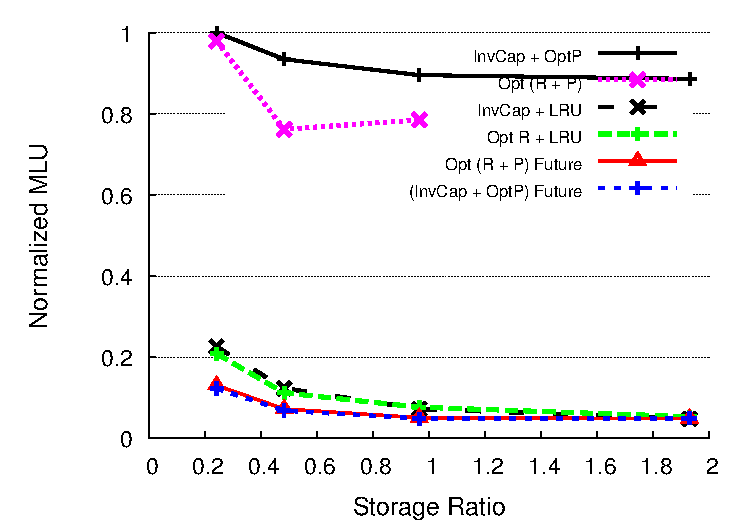
\includegraphics[scale=0.5]{graphSet1/shortvideos/storageAbilene.pdf}
}
\subfigure[US-ISP]{
	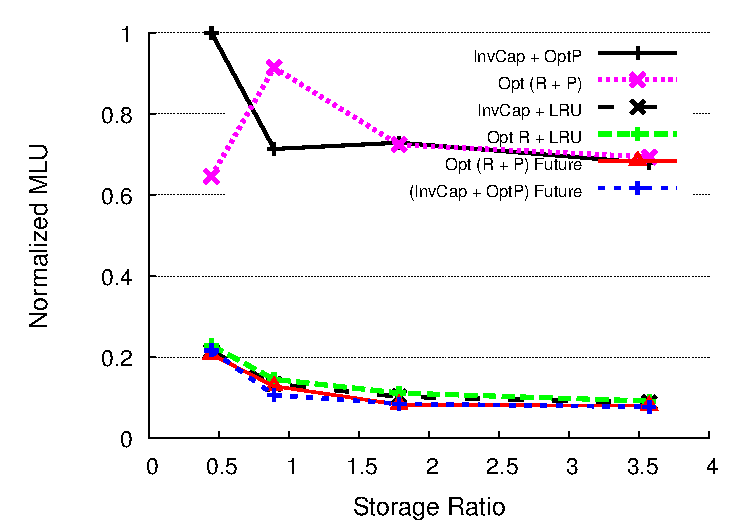
\includegraphics[scale=0.5]{graphSet1/shortvideos/storageATT.pdf}
}
\end{center}
\vspace{-0.2in}
\caption{News videos trace. \invlru\ scheme  outperforms \optrp\ scheme by an order of magnitude on both topologies because approx 50\% of requests each day are for the new content added on that day.}
\label{fig:newsMLU}
\end{figure}

\begin{figure}[t]
\begin{center}
\subfigure[Abilene]{
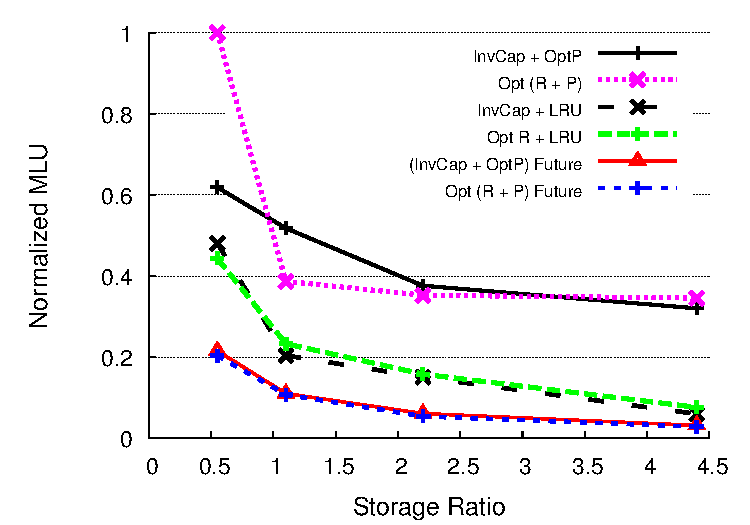
\includegraphics[scale=0.5]{graphSet1/lruecmp3/AbileneVideos.pdf}
%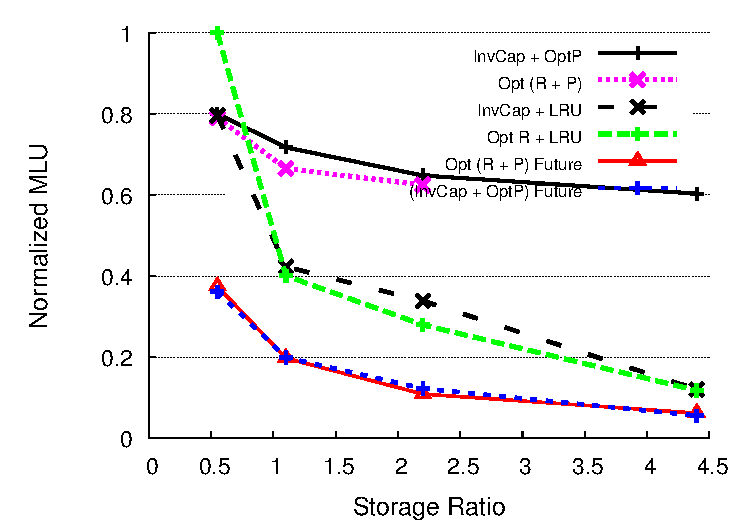
\includegraphics[scale=0.5]{graphSet1/tvAll/storageAbilene.pdf}
%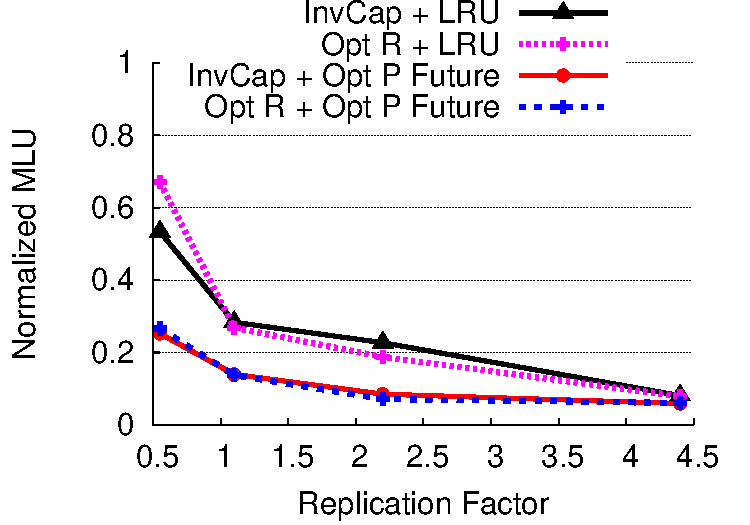
\includegraphics[scale=0.5]{graphSet1/tvAll/storageAbilene2_Xiaozheng.pdf}
}
  \subfigure[US-ISP]{
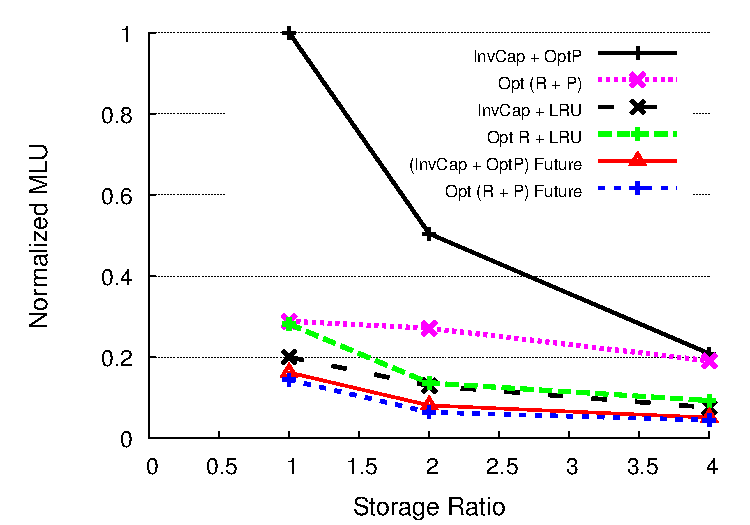
\includegraphics[scale=0.5]{graphSet1/lruecmp3/ATTVideos.pdf}
%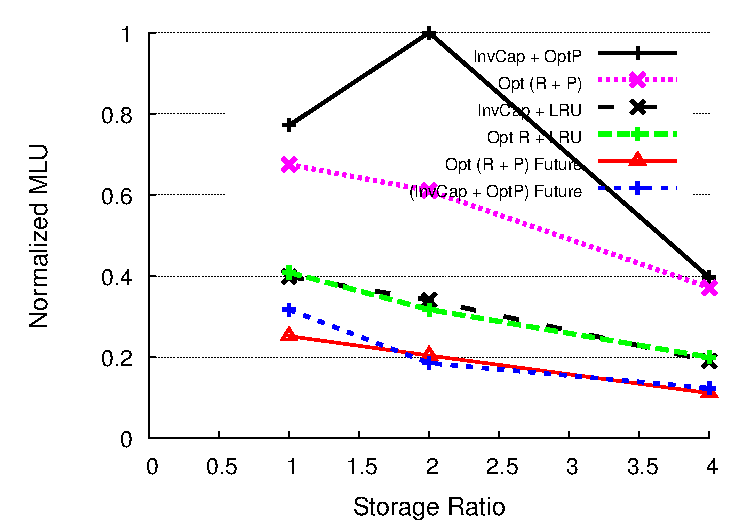
\includegraphics[scale=0.5]{graphSet1/tvAll/storageATT.pdf}
}
\end{center}
\vspace{-0.2in}
\caption{Entertainment Videos trace. \invlru\ performs better than a \optrp\  scheme by a factor of 9$\times$ and 4$\times$ on Abilene and US-ISP topologies.  }
\label{fig:entertainmentMLU}
\end{figure}

\begin{figure}[t]
\begin{center}
\subfigure[Abilene]{
	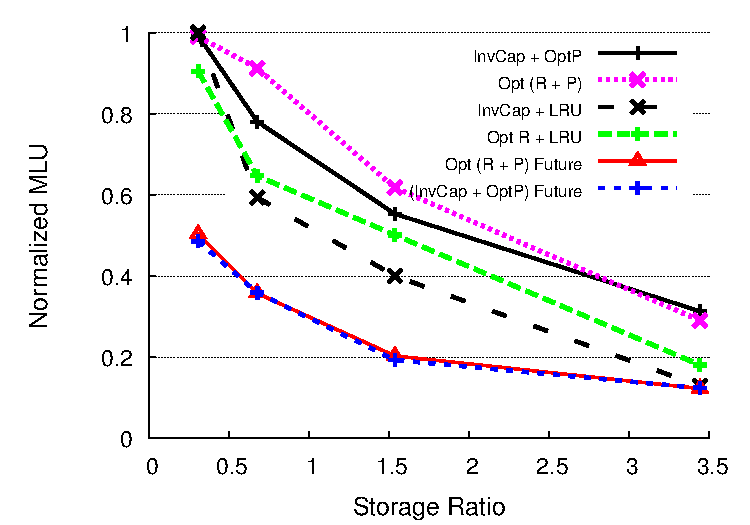
\includegraphics[scale=0.5]{graphSet1/software/storageAbilene.pdf}
}
\subfigure[US-ISP]{
	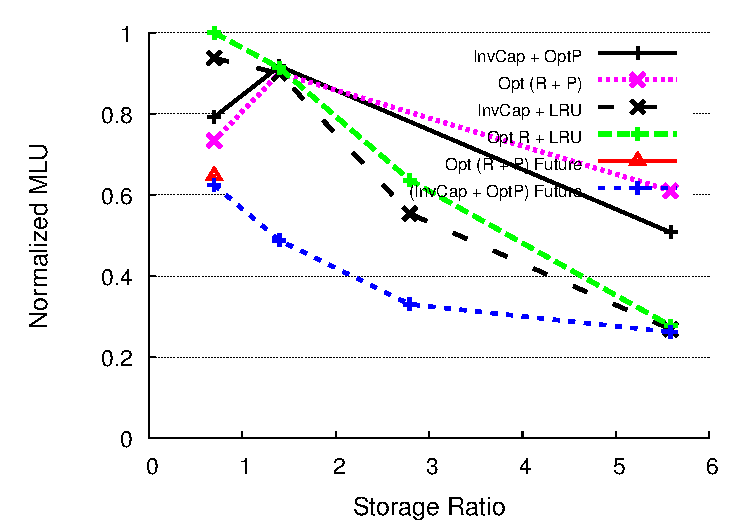
\includegraphics[scale=0.5]{graphSet1/software/storageATT.pdf}
}
\end{center}
\vspace{-0.2in}
\caption{Downloads trace.  \optrp\ performs poorly because of multiple new popular software downloads on one day of the trace.  \invlru\ performs well on both traces. It performs close to \optrpfuture\  on the Abilene topology and is only 15\% worse compared to \optrpfuture\ on the  US-ISP trace.}
\label{fig:softwaredownloads}
\end{figure}

\begin{wrapfigure}[12]{r}{2.3in}
\centering
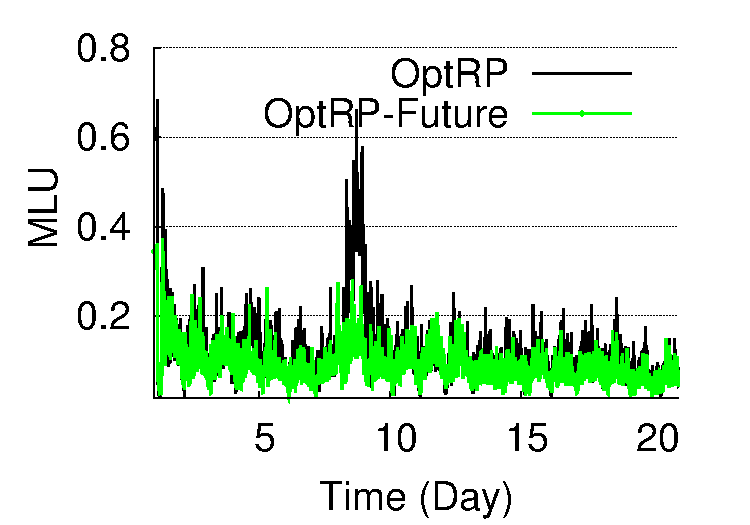
\includegraphics[scale=0.5]{graphSet1/software/mlu_Xiaozheng.pdf}
\end{wrapfigure}

% END OF EAT
}




% NEW SET OF GRAPHS





\begin{figure*}[t]
\begin{center}
\subfigure[News,  US-ISP] {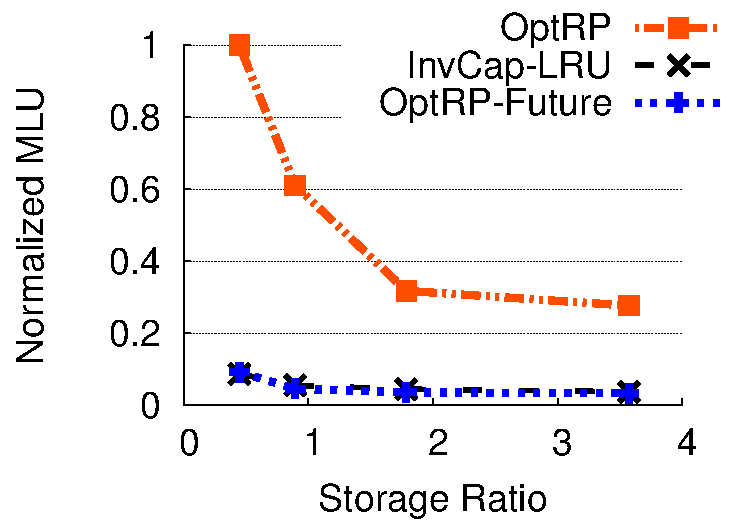
\includegraphics[scale=0.45]{graphSet1/newmaingraphs/ATTNews.pdf}}
\subfigure[Entertainment,  US-ISP] {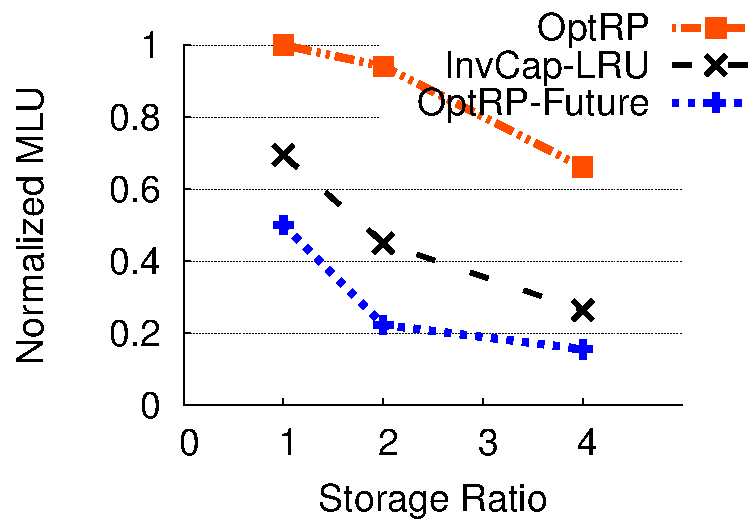
\includegraphics[scale=0.45]{graphSet1/newmaingraphs/ATTVideos.pdf}}
\subfigure[Downloads,  US-ISP] {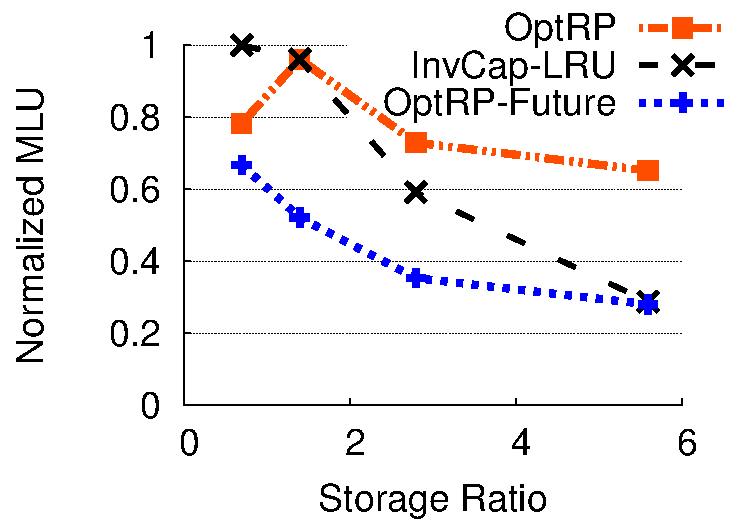
\includegraphics[scale=0.45]{graphSet1/newmaingraphs/ATTDownloads.pdf}}
\subfigure[News,  Abilene] {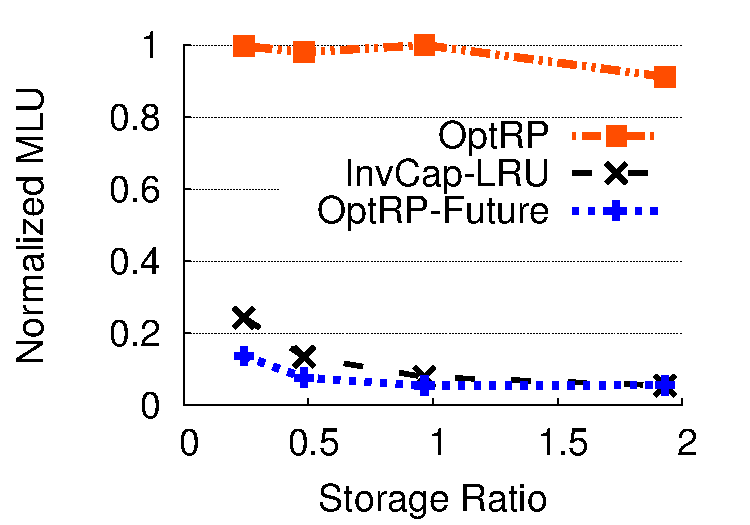
\includegraphics[scale=0.45]{graphSet1/newmaingraphs/AbileneNews.pdf}}
\subfigure[Entertainment,  Abilene] {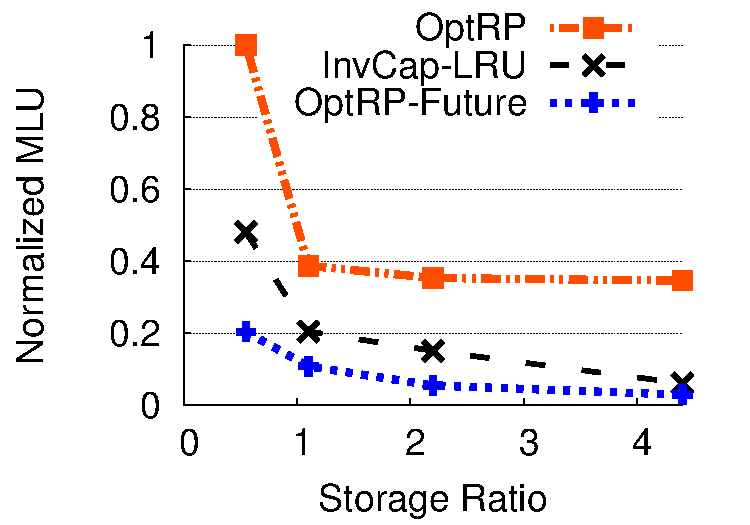
\includegraphics[scale=0.45]{graphSet1/newmaingraphs/AbileneVideos.pdf}}
\subfigure[Downloads,  Abilene] {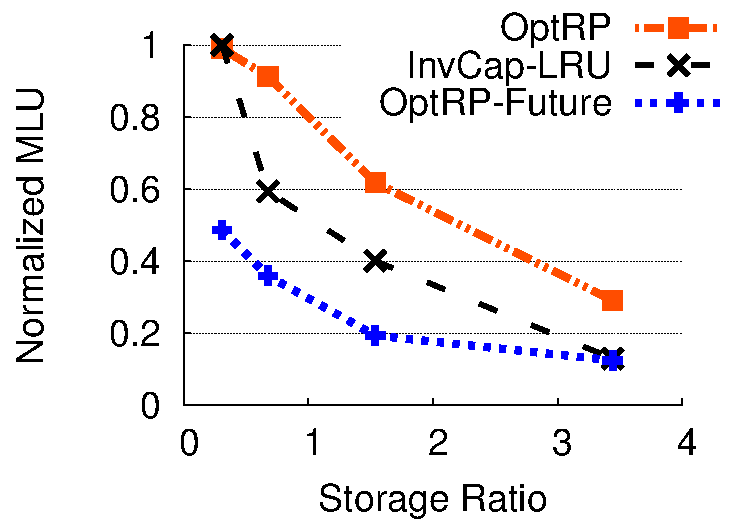
\includegraphics[scale=0.45]{graphSet1/newmaingraphs/AbileneDownloads.pdf}}
\end{center}
\vspace{-0.2in}
\caption{\Planned\ \optrp\ performs much worse than \unplanned\  \invlru. \optrpfuture\ performs moderately better than \invlru\ primarily at small storage ratios.}
\vspace{-0.1in}
\label{fig:newmaingraphs}
\end{figure*}



\begin{figure}[t]	
\begin{center}
\subfigure[News,  Abilene]{
	%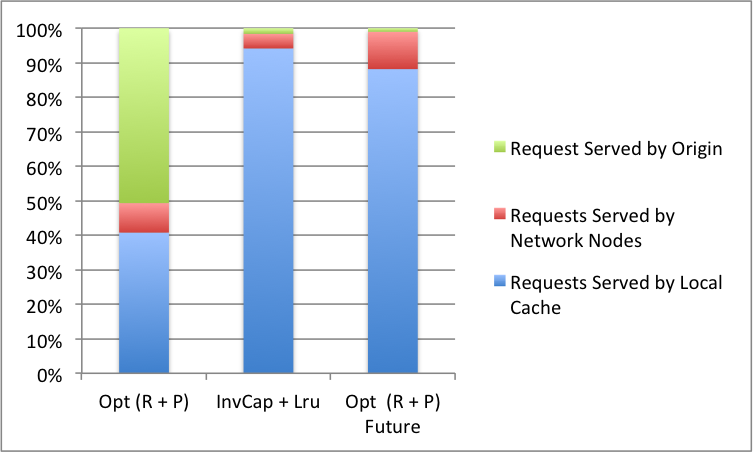
\includegraphics[width=0.2\textwidth]{graphSet1/shortvideos/AbileneNews.png}
	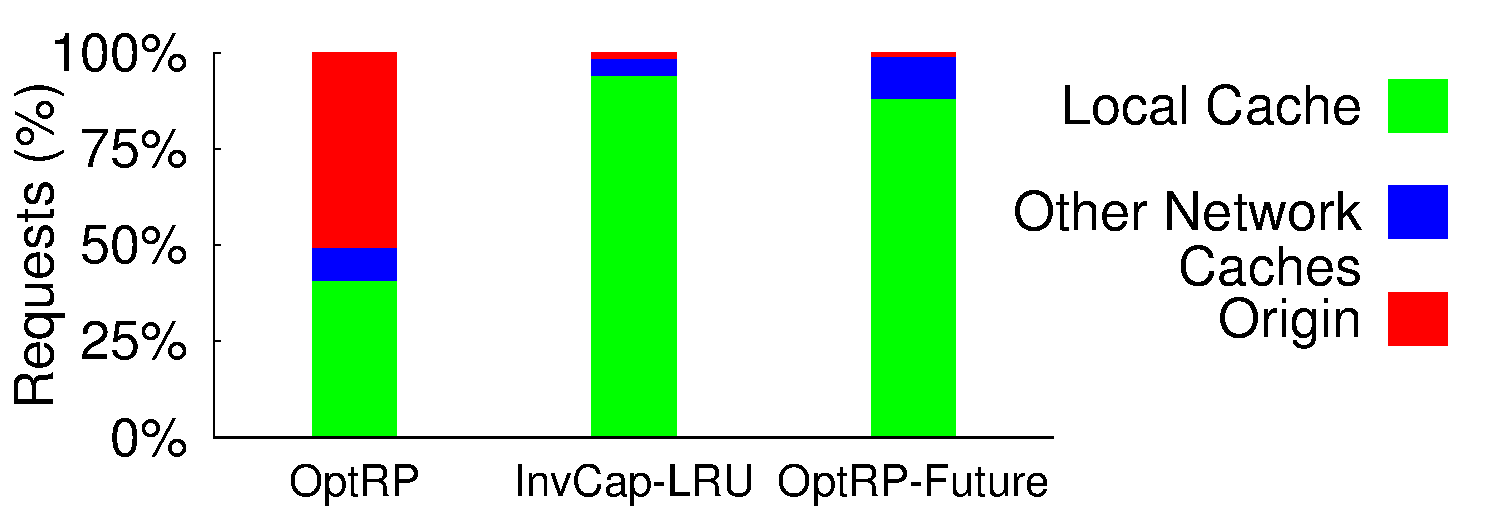
\includegraphics[width=0.45\textwidth]{graphSet1/shortvideos/Newsbar_Xiaozheng.pdf}
}
\subfigure[Entertainment,  Abilene]{
	%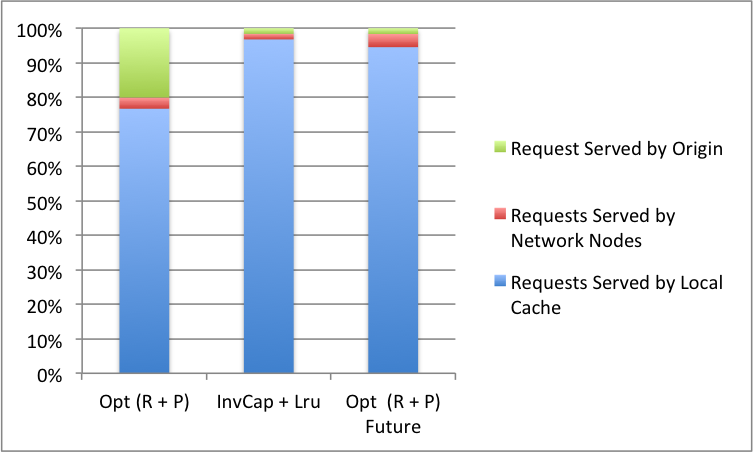
\includegraphics[width=0.2\textwidth]{graphSet1/tvAll/AbileneVideos.png}
	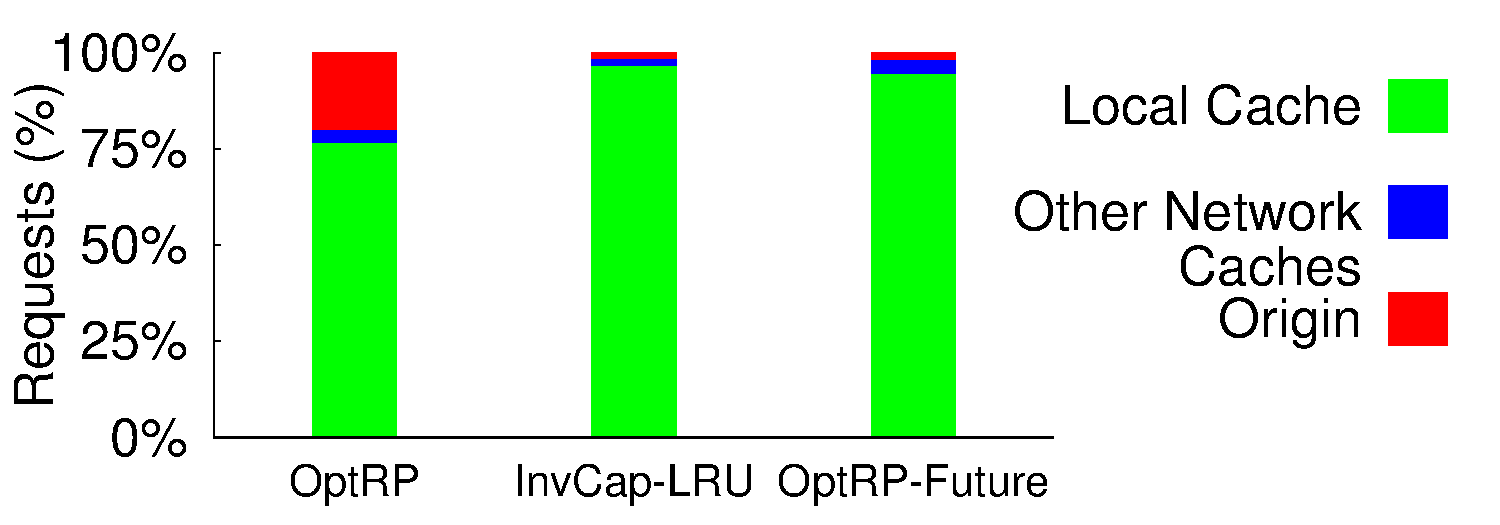
\includegraphics[width=0.45\textwidth]{graphSet1/tvAll/Videobar_Xiaozheng.pdf}
}
\end{center}
\vspace{-0.2in}
\caption{[Videos, Abilene] \optrp\ serves 50\%  and 21\% of news and entertainment requests respectively from the origin. \invlru\ and \optrpfuture\ serve at most 2\% from the origin.}
\vspace{-0.15in}
\label{fig:originrequest}
\end{figure}
%Fraction of requests served from local cache, other network caches and origin. 


\begin{figure}[t]
\begin{center}
	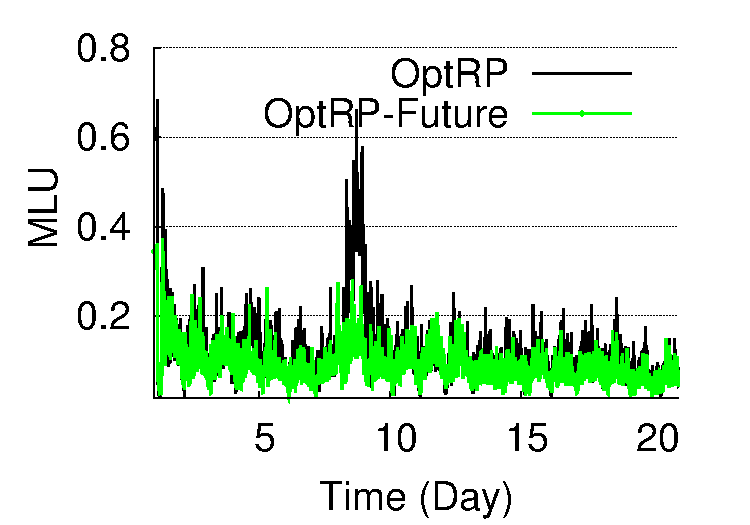
\includegraphics[scale=0.45]{graphSet1/software/mlu_Xiaozheng.pdf}
\end{center}
\vspace{-0.30in}
%\caption{Comparison of MLU of \optrp\ and \optrpfuture\ on downloads trace, US-ISP.}
\caption{[Downloads, US-ISP] \optrp\ incurs a very high MLU on one ``peak load'' day.}
%\vspace{-0.3in}
\label{fig:softwarepeak}
\end{figure}

%Content popularity is predictable on most days based on previous day, hence \optrp\  performs well. Due to multiple new popular  software updates on day 8, a \optrp\  notices a sharp increase in MLU compared to other days in the trace.


\begin{figure*}[t]	
\begin{center}
\subfigure[MLU reduction  with \optlru\ compared to \invlru]{
	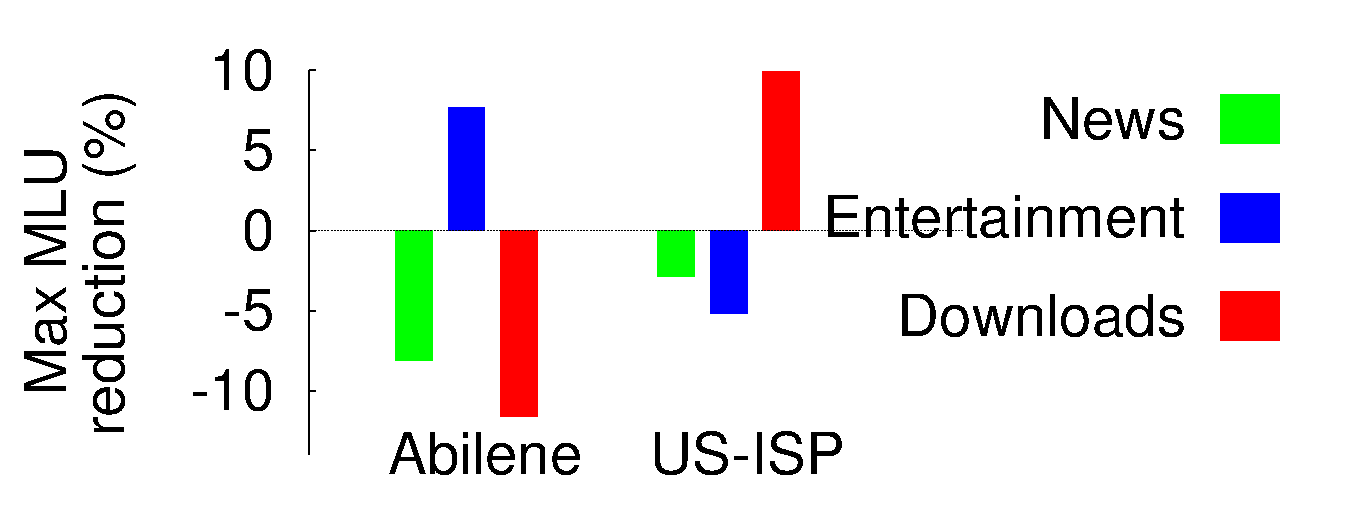
\includegraphics[width=0.4\textwidth]{graphSet1/mlureduction/inv-optr.pdf}
}
\subfigure[MLU reduction with \optrpfuture\ compared to \invoptpfuture]{
	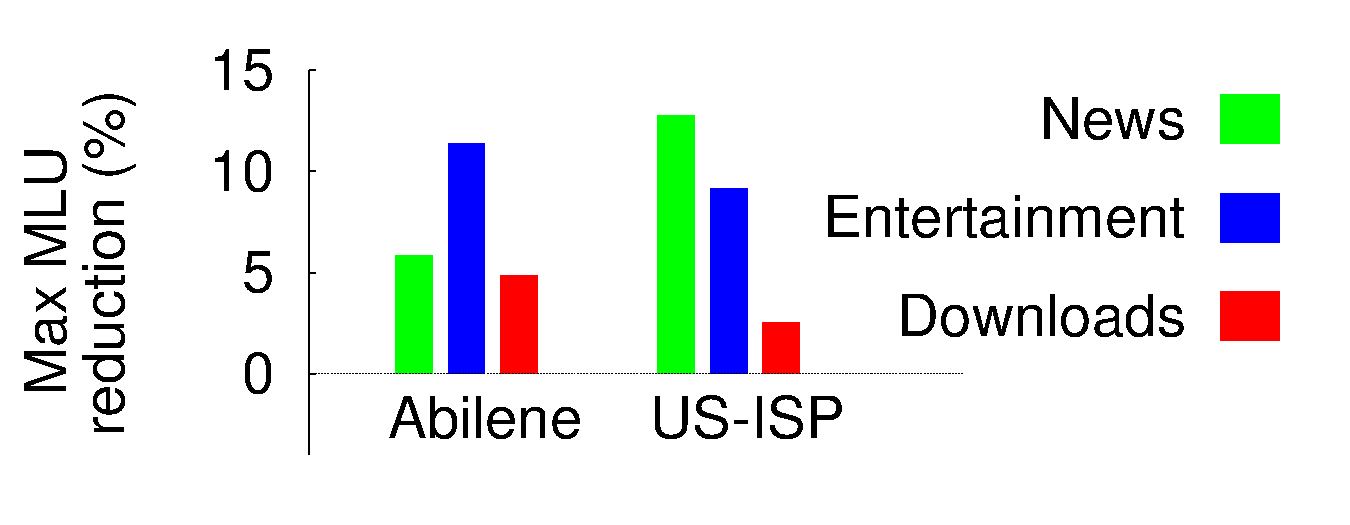
\includegraphics[width=0.4\textwidth]{graphSet1/mlureduction/inv-optr-future.pdf}
}
\end{center}
\vspace{-0.25in}
\caption{[All traces] Optimizing routing yields little  improvement to MLU of either \invlru\ or \invoptpfuture}\vspace{-0.2in}
\label{fig:mlureduction}
\end{figure*}

\subsection{Comparison of network cost}

\subsubsection{Analysis of video \& downloads traffic}
\label{sec:videodownload}


Figure \ref{fig:newmaingraphs} shows the results for the news, entertainment and downloads traces on  Abilene and US-ISP. Our first observation is that a realistic \planned\  placement and routing scheme, \optrp, performs significantly worse than a completely \unplanned\  scheme, \invlru. \optrp\ has   2.2$\times$ to 17$\times$ higher MLU than \invlru\ even at the maximum storage ratio in each graph.  \optrp\ has a high MLU because it optimizes routing and placement based on the previous day's content demand while a significant fraction of requests are for new content not accessed the previous day (see Figure \ref{fig:akamaichurn}).  Due to new content, the incoming traffic from origin servers  is significant, so the utilization of links near the exit nodes connecting to the origin servers is extremely high. 

%Even when storage ratio is increased, \optrp\ continues to serve the requests for new content not accessed the previous day from  origin servers and performs poorly.

The fraction of requests served from the origin is much higher for \optrp\ compared to \invlru\ and \optrpfuture\  on the news and the entertainment traces. Figure  \ref{fig:originrequest} shows that  \optrp\  serves  50\% and 21\% of requests from the origin for news   and entertainment respectively. In comparison, \invlru\ and \optrpfuture\ serve less than 2\% of requests from the origin. Therefore, \optrp\ has a much higher MLU than both  \invlru\ and \optrpfuture\ on the two traces. 

The downloads trace differs from other traces in that, except for one day, the traffic is quite predictable based on the previous day's history. This is reflected in the performance of \optrp\ that performs nearly the same as \optrpfuture\ on all days except the ninth day of the trace (see Figure \ref{fig:softwarepeak}). The surge in MLU for \optrp\ on the ninth day is because nearly 20\% of requests on this day is for new content consisting of highly popular software update releases (see Figure \ref{fig:akamaichurn}). The surge in MLU on this one day is mainly responsible for the poor performance of \optrp\ on the downloads trace.

%On other days, the traffic quite predictable based on the previous day's history as only 2-3\% of requests are for new content, and therefore \optrp\ matches the performance of \optrpfuture.

%On downloads trace, \optrp\  performs nearly the same as \optrpfuture\ on all days except the ninth day of the trace (see Figure \ref{fig:softwarepeak}). 

%
%New content published each day needs to be fetched from the origin which increases utilization of links near the exit nodes of the network in transit to the origin. 
%
%which leads to  a high MLU when 
% and a significant fraction of requests in both the traces, especially the news trace, are for new content not accessed the previous day
%
%\optrp\ does poorly because it has a high MLU on those days on which a significant fraction of requests are for new content not accessed the previous day. As \optrp\ calculates routing based on previous day's demand, new content increases the ``miss'' traffic due to content 
%
% it calculates routing and placement based on previous day's content demand and   has a high MLU on the days when a significant fraction of requests are for new content not accessed the previous day.
%
%but a significant fraction of requests each day are for new content not published the previous day. 
%
%
%\optrp\ is disadvantaged  in having to optimize routing and placement without knowledge of future demand and a significant fraction of requests in both the traces, especially the news trace, are for new content not accessed the previous day. This increases the ``miss traffic'' for content not present in cache that have to be fetched from origin. In particular, this leads to increased utilization of links near the exit nodes of the network in transit to the origin. 
%
%
%Figure \ref{fig:originrequest} shows that \optrp\  serves  50\% and 21\% of requests from the origin servers for the news trace  and entertainment trace respectively while \invlru\ and \optrpfuture\ serve less than 2\% of requests from the origin servers. Therefore, both  \invlru\ and \optrpfuture\  have a significantly lower MLU and hence lower network cost.
%


%\optrp\ is disadvantaged  in having to optimize routing and placement without knowledge of future demand and a significant fraction of requests in both the traces, especially the news videos, are for new content not accessed the previous day. This increases the ``miss traffic'' for content not present in cache that have to be fetched from another node or origin. In particular, this leads to increased utilization of links near the exit nodes of the network in transit to the origin. Figure \ref{fig:originrequest} shows that \optrp\  serves  50\% and 21\% of requests from the origin servers for the news trace  and entertainment trace respectively while \invlru\ and \optrpfuture\ serve less than 2\% of requests from the origin servers. Therefore, both  \invlru\ and \optrpfuture\  have a significantly lower MLU and hence lower network cost.

%But, a deeper analysis of the downloads traces show that the difference between \invcap\ and \optrp\ is primarily due to one day of traffic in the trace when major new software updates appear to have been released. These account for 20\% of all requests during the day. This results in a sharp increase in MLU for \optrp\ as shown in Figure \ref{fig:softwarepeak}. 
%As can be visually discerned from the figure, both  \optrp\  and  \optrpfuture\ perform nearly the same on other days in the trace.  This shows that the download traffic quite predictable based on the previous day's history, barring highly popular software download releases. 

% This contrasts with our results for video traffic traces where we observed on average  20\% requests for new content in  the entertainment trace and more than 50\% in the news trace. 


%
%\begin{SCfigure}[t]
%\subfigure[Content chunking improves performance of \invlru\ relative to \optrpfuture. Entertainment trace, ATT] {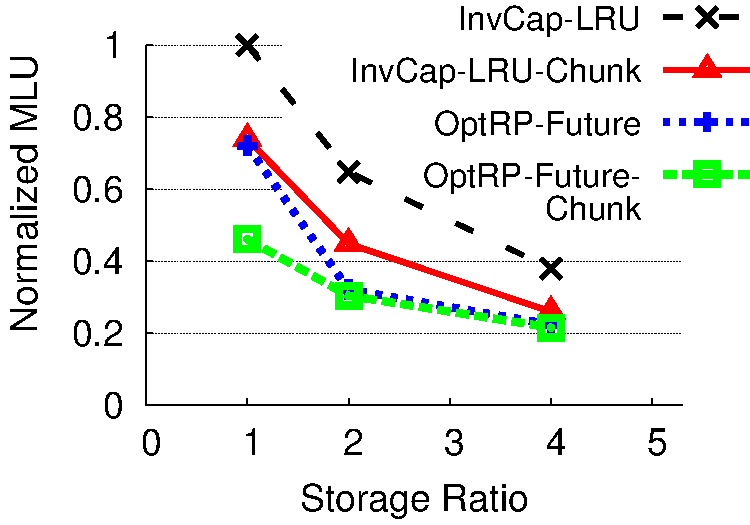
\includegraphics[scale=0.45]{graphSet1/chunkcomp/ATTVideos.pdf}}
%\subfigure[Hybrid placement strategies either perform as well as \invlru\ or worse for both traces. Entertainment trace, Abilene] {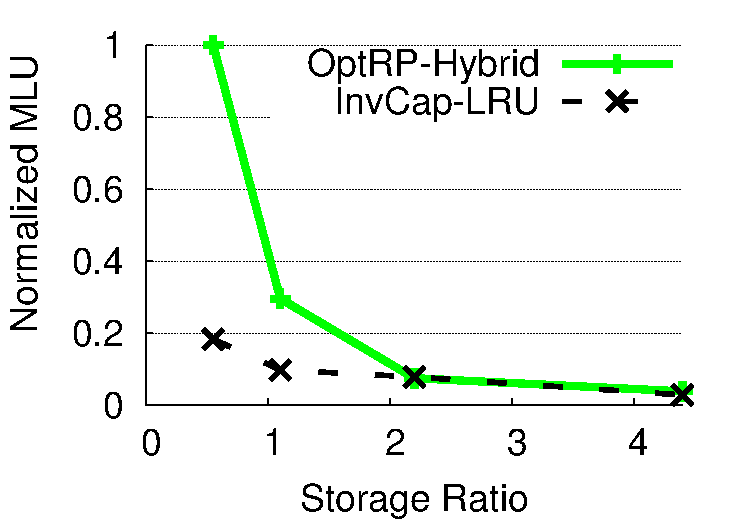
\includegraphics[scale=0.45]{graphSet1/hybrid/AbileneVideos.pdf}}
%\subfigure[\optrp\ matches the performance of \invlru\ if placement and routing is updated eight times per day. Entertainment trace, ATT] {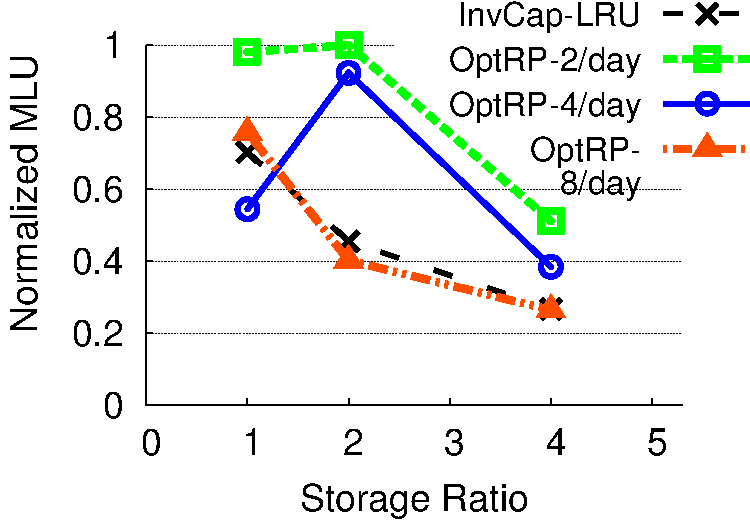
\includegraphics[scale=0.45]{graphSet1/tefrequency/ATTVideos.pdf}}
%\vspace{-0.35in}
%\label{fig:newmaingraphs2}
%\end{SCfigure}



\eat
{
The relative difference between  \invlru\ and \optrp\ grows larger as storage ratio increases. This is because \invlru\  utilizes the additional cache at each location to increase its hit rate and thereby reduce the traffic on congested links in the network. On the other hand, \optrp\ continues to serve the requests for new content not accessed the previous day from the origin and does poorly even if the storage ratio increases. 
}

%\optrp\ continues to serve the requests for new content from the origin server even at higher storage ratios with little improvement.

% invlru performs significantly better than 
Next, we observe that \invlru\ does underperform compared to \optrpfuture\ that has knowledge of future content demand. However, \invlru\ improves with respect to \optrpfuture\ as the storage ratio increases.  The maximum difference between the two schemes is for the experiment with entertainment trace on US-ISP topology. In this case, at a storage ratio of 1,  \invlru\ has twice the MLU of the \optrpfuture\ scheme; the difference reduces to 1.6$\times$ at a storage ratio of 4. This shows that when storage is scarce, \planned\  placement with future knowledge can significantly help by using knowledge of the global demand to maximize the utility of the storage. However, if storage is plentiful, the relative advantage of \optrpfuture\ is smaller. An important implication of our results is that \ancp\ should attempt to do \planned\  placement only if the future demand can be accurately known or estimated. Otherwise, a simpler \unplanned\  scheme such as LRU suffices.   

%\textcolor{blue}
%{
%At this point, our analysis does not account for the effect of content chunking, which further reduces the difference between \invlru\ and \optrpfuture\ (Section \ref{sec:chunking}).
%}

% \invlru\ performs better with respect to \optrpfuture\ on the news video trace compared to the entertainment trace because the entertainment trace consists of large files such as TV shows and movies along with small files, which cause a large number of cache evictions when a large object is inserted into the LRU cache. The news trace consist of a high fraction ($> 95\%$) of short video clips ($< 10$ min) and hence does not face the same problem.




%To answer this question, we compared \invlru\ with  \optlru\ and \optrpfuture\ with \invoptpfuture. 
How are the above conclusions impacted if  \invlru\  were to optimize routing or   \optrpfuture\  were to use InvCap routing? To answer this question, we analyze the maximum reduction in MLU by using \optlru\ over \invlru\ across all storage ratios in Figure  \ref{fig:mlureduction}. We similarly compare \optrpfuture\ and \invoptpfuture.   We find that \optlru\ improves the MLU over  \invlru\ by at most 10\% across all traces suggesting that optimizing routing is of little value for an \unplanned\  placement scheme.   \optrpfuture\  reduces the network cost by at most 13\% compared to \invoptpfuture. As we consider \optrpfuture\ to be the ``ideal'' scheme with full future knowledge, these results show that the best MLU can be achieved by optimizing content placement alone; optimizing routing adds little additional value.

%We present the results for this experiment for both traces in Figures \ref{fig:newsMLU} and \ref{fig:entertainmentMLU}.

%We present the results for this experiment for both traces in Figures \ref{fig:newsMLU} and \ref{fig:entertainmentMLU}.

% Another important difference between \invlru\ and \optrpfuture\ is that the former scheme does not optimize routing in the network while the latter does. A natural question is if this difference is important. That is, if  \invlru\  were to optimize routing or   \optrpfuture\  were to use \invcap\ routing, does it change any of our conclusions? 






%We have seen that \invlru\ performs significantly better than a realistic demand aware scheme. This raises the question whether a better content placement and routing strategy exists. The comparison of \optrpfuture\ and \invlru\ shows that the former scheme indeed does perform better, more so at smaller replication factors. 
%But the performance of \invlru\ improves with respect to \optrpfuture, as replication factor increases in the network.  For example for the US-ISP topology we find that at a replication factor of 1, \invlru\ has twice the network of the \optoptfuture\ scheme. 

%At higher replication factors, the relative difference between the two scheme reduces which shows that 


 
Somewhat counterintuitively, the MLU sometimes increases with a higher storage ratio for the \optrp\ scheme. There are three reasons that explain this. First, the optimization formulation optimizes for the content matrix assuming that the demand is uniformly spread across the entire day, however the requests may actually arrive in a bursty manner. So it may be sub-optimal compared to a scheme that is explicitly optimized for a known sequence of requests. Second,  the optimization formulation optimizes the MLU for the ``smoothed'' matrix, but the set of objects placed by the optimal strategy with more storage may not necessarily be a superset of the objects placed by the strategy with lesser storage at any given PoP. Third, and most importantly, the actual content matrix for the next day may differ significantly from that of the previous day. All of these reasons make the so-called ``optimal'' \optrp\ strategy suboptimal and in combination are responsible for the nonmonotonicity observed in the experiments.





\eat{
\subsubsection{Analysis of Video Traffic}
\label{sec:video}

We present our results for the two video traces--news and entertainment--on Abilene and US-ISP topologies.  Figure \ref{fig:newsMLU} and Figure \ref{fig:entertainmentMLU}  show the results for the news and entertainment traces respectively.

%\tbd{I will replot the graphs Figure \ref{fig:newsMLU} and Figure \ref{fig:entertainmentMLU}. These graphs will only have three line \invlru, \optrp, \optrpfuture}
We first draw attention the performance of a realistic \planned\  placement and routing scheme, \optrp, compared to a completely \unplanned\  scheme. Surprisingly, we find that that \optrp\ performs significantly worse than \invlru\  for both traces and topologies. The MLU of  \optrp's is worse than  \invlru\  by a 2$\times$ to 10$\times$ factor  depending on the trace and the storage ratio. 

\optrp\ is disdvantaged  in having to optimize routing and placement without knowledge of future demand and a significant fraction of requests in both the traces, especially the news videos, are for new content not accessed the previous day. This increases the ``miss traffic'' for content not present in cache that have to be fetched from another node or origin. In particular, this leads to increased utilization of links near the exit nodes of the network in transit to the origin. Figure \ref{fig:originrequest} shows that \optrp\  serves  50\% and 21\% of requests from the origin servers for the news trace  and entertainment trace respectively while \invlru\ and \optrpfuture\ serve less than 2\% of requests from the origin servers. Therefore, both  \invlru\ and \optrpfuture\  have a significantly lower MLU and hence lower network cost.
 

The relative difference between the \invlru\ and \optrp\ grows larger as storage ratio increases in the network. This is because \invlru\ is able to dynamically cache new content and utilize the additional cache at each location to increase its hit rate and thereby reduce the traffic on congested links in the network. On the other hand, \optrp, does not effectively deal with the new content that was not accessed the previous day and does poorly even if the storage ratio increases. \optrp\ continues to serve the requests for new content from the origin server even at higher storage ratios with little improvement.
 
% invlru performs significantly better than 
Next, we observe that \invlru\ does underperform \optrpfuture\ that has knowledge of future content demand. However, \invlru\ improves with respect to \optrpfuture\ as the storage ratio increases.  The maximum difference between the two schemes is for the experiment with entertainment trace on US-ISP topology. In this case, at a storage ratio of 1,  \invlru\ has twice the MLU of the \optrpfuture\ scheme; the difference reduces to 1.6 $\times$ at a storage ratio of 4. This shows that when storage is scarce, \planned\  placement with future knowledge can significantly help by using knowledge of the global demand to maximize the utility of the storage. However, if storage is plentiful, the relative advantage of \optrpfuture\ is smaller. An important implication of our results is that an \ncp\ should attempt to do \planned\  placement only if the future demand can be accurately known or estimated. Otherwise, a simpler demand-oblivious scheme such as LRU suffices.

% \invlru\ performs better with respect to \optrpfuture\ on the news video trace compared to the entertainment trace because the entertainment trace consists of large files such as TV shows and movies along with small files, which cause a large number of cache evictions when a large object is inserted into the LRU cache. The news trace consist of a high fraction ($> 95\%$) of short video clips ($< 10$ min) and hence does not face the same problem.

Another important difference between \invlru\ and \optrpfuture\ is that the former scheme does not optimize routing in the network while the latter does. A natural question is if this difference is important. That is, if  \invlru\  were to optimize routing or   \optrpfuture\  were to use \invcap\ routing, does it change any of our conclusions? To answer this question, we compared \invlru\ with the \optlru\ and \optrpfuture\ with \invoptpfuture.   We present the results for this experiment for both traces in Figures \ref{fig:newsMLU} and \ref{fig:entertainmentMLU}.
We find that \optlru\ does not improve the MLU over  \invlru\ in any of the traces suggesting that optimizing routing is of little value for a demand-oblivious content placement scheme.  Furthermore, \optrpfuture\  and \invoptpfuture\ perform nearly identically in  all experiments, except for the experiment with the entertainment trace on the US-ISP network. In this experiment as well, the difference between these schemes becomes negligible at storage ratio of 4. As we consider \optrpfuture\ to be the ``ideal'' scheme with full future knowledge, these results show that the best MLU can be achieved by optimizing content placement alone; optimizing routing adds little additional value.





%We have seen that \invlru\ performs significantly better than a realistic demand aware scheme. This raises the question whether a better content placement and routing strategy exists. The comparison of \optrpfuture\ and \invlru\ shows that the former scheme indeed does perform better, more so at smaller replication factors. 
%But the performance of \invlru\ improves with respect to \optrpfuture, as replication factor increases in the network.  For example for the US-ISP topology we find that at a replication factor of 1, \invlru\ has twice the network of the \optoptfuture\ scheme. 

%At higher replication factors, the relative difference between the two scheme reduces which shows that 

 
Somewhat counterintuitively, the MLU sometimes increases with a higher storage ratio for the \optrp\ scheme. There are three reasons that explain this. First, the optimization formulation optimizes for the content matrix assuming that the demand is uniformly spread across the entire day, however the requests may actually arrive in a bursty manner. So it may be sub-optimal compared to a scheme that is explicitly optimized for a known sequence of requests. Second,  the optimization formulation optimizes the MLU for the ``smoothed'' matrix, but the set of objects placed by the optimal strategy with more storage may not necessarily be a superset of the objects placed by the strategy with lesser storage at any given PoP. Third, and most importantly, the actual content matrix for the next day may differ significantly from that of the previous day. All of these reasons make the so-called ``optimal'' \optrp\ strategy suboptimal and in combination are responsible for the nonmonotonicity observed in the experiments.





\subsubsection{Analysis of Downloads}
\label{sec:downloads}
%In this section, we present our results for the software downloads trace highlighting the unique traffic characteristics of software downloads traffic. 
%\tbd{- need to write dates are for the other two traces ?}
%Our traces for software download traffic span from 5 Dec 2010 to 25 Dec 2010. 

Figure \ref{fig:softwaredownloads} shows the results of our experiments for the downloads traces.  

Our main findings from the prior section for videos, namely--\invlru\ performs significantly better than \optrp; \optrpfuture\ performs better than  \invlru; and optimizing routing adds little value;--remain unchanged for the downloads traffic.
But, a deeper analysis of the downloads traces show that the difference between \invcap\ and \optrp\ is primarily due to one day of traffic in the trace when major new software updates appear to have been released. These account for 20\% of all requests during the day. This results in a sharp increase in MLU for \optrp\ as shown in Figure \ref{fig:softwarepeak}. 

As can be visually discerned from the figure, both  \optrp\  and  \optrpfuture\ perform nearly the same on other days in the trace.  This shows that the download traffic quite predictable based on the previous day's history, barring highly popular software download releases.  This contrasts with our results for video traffic traces where we observed on average  20\% requests for new content in  the entertainment trace and more than 50\% in the news trace. 

In fact, we find that downloads traffic has a substratum of highly-predictable traffic (example, hourly or daily anti-virus updates) with episodes of large events (such as a major OS releases). One could argue that if the major events are knowable in advance, an \ncp\ can pursue a demand-aware placement with future knowledge and achieve results closer to \invoptpfuture\ (say) that does up to 33\% better than demand-oblivous LRU. 

Lastly, we reiterate our observation from the video traces that whether or not routing is optimized makes only a small difference to the MLU in all cases. As Figure \ref{fig:softwaredownloads} shows, \optlru\ does not improve the MLU over   \invlru, neither does  \invoptpfuture\ worsen the MLU for   \optrpfuture. 
}




% 
%
% 
%  and comes close to achieving the seemingly unrealistic \optrpfuture\ scheme on increasing the replication factor in the network.  The maximum difference between \invlru\ and \optrpfuture\ is for the experiment with entertainment  trace on the US-ISP topology. In that case, the difference between \invlru\ and \optopt\ 
%
%
%For small replication factors, \optrpfuture\  can improve the network cost over \invlru\ by a factor of up to 2$\times$ but the difference between the two reduces considerably on increasing the replication factor.  The maximum difference between the two schemes is for the 
%
%In the entertainment videos trace on US-ISP topology, the difference between \invlru\ and \optrpfuture\ reduces considerably on increasing the replication from 
%
%
%, but the difference 
%   but the difference between them reduces consider
%The performance of \invlru\  improves considerably on increasing the replication factor.  This is because cache size at each PoP increases with 
%
%This can easily be explained based 
%The relative difference between \invlru\ and \optrpfuture\  
%
%Surprisingly, a demand oblivious routing and demand oblivious placement performs 












%\begin{figure*}
%\begin{center}
%\subfigure[Churn Metric]{
%	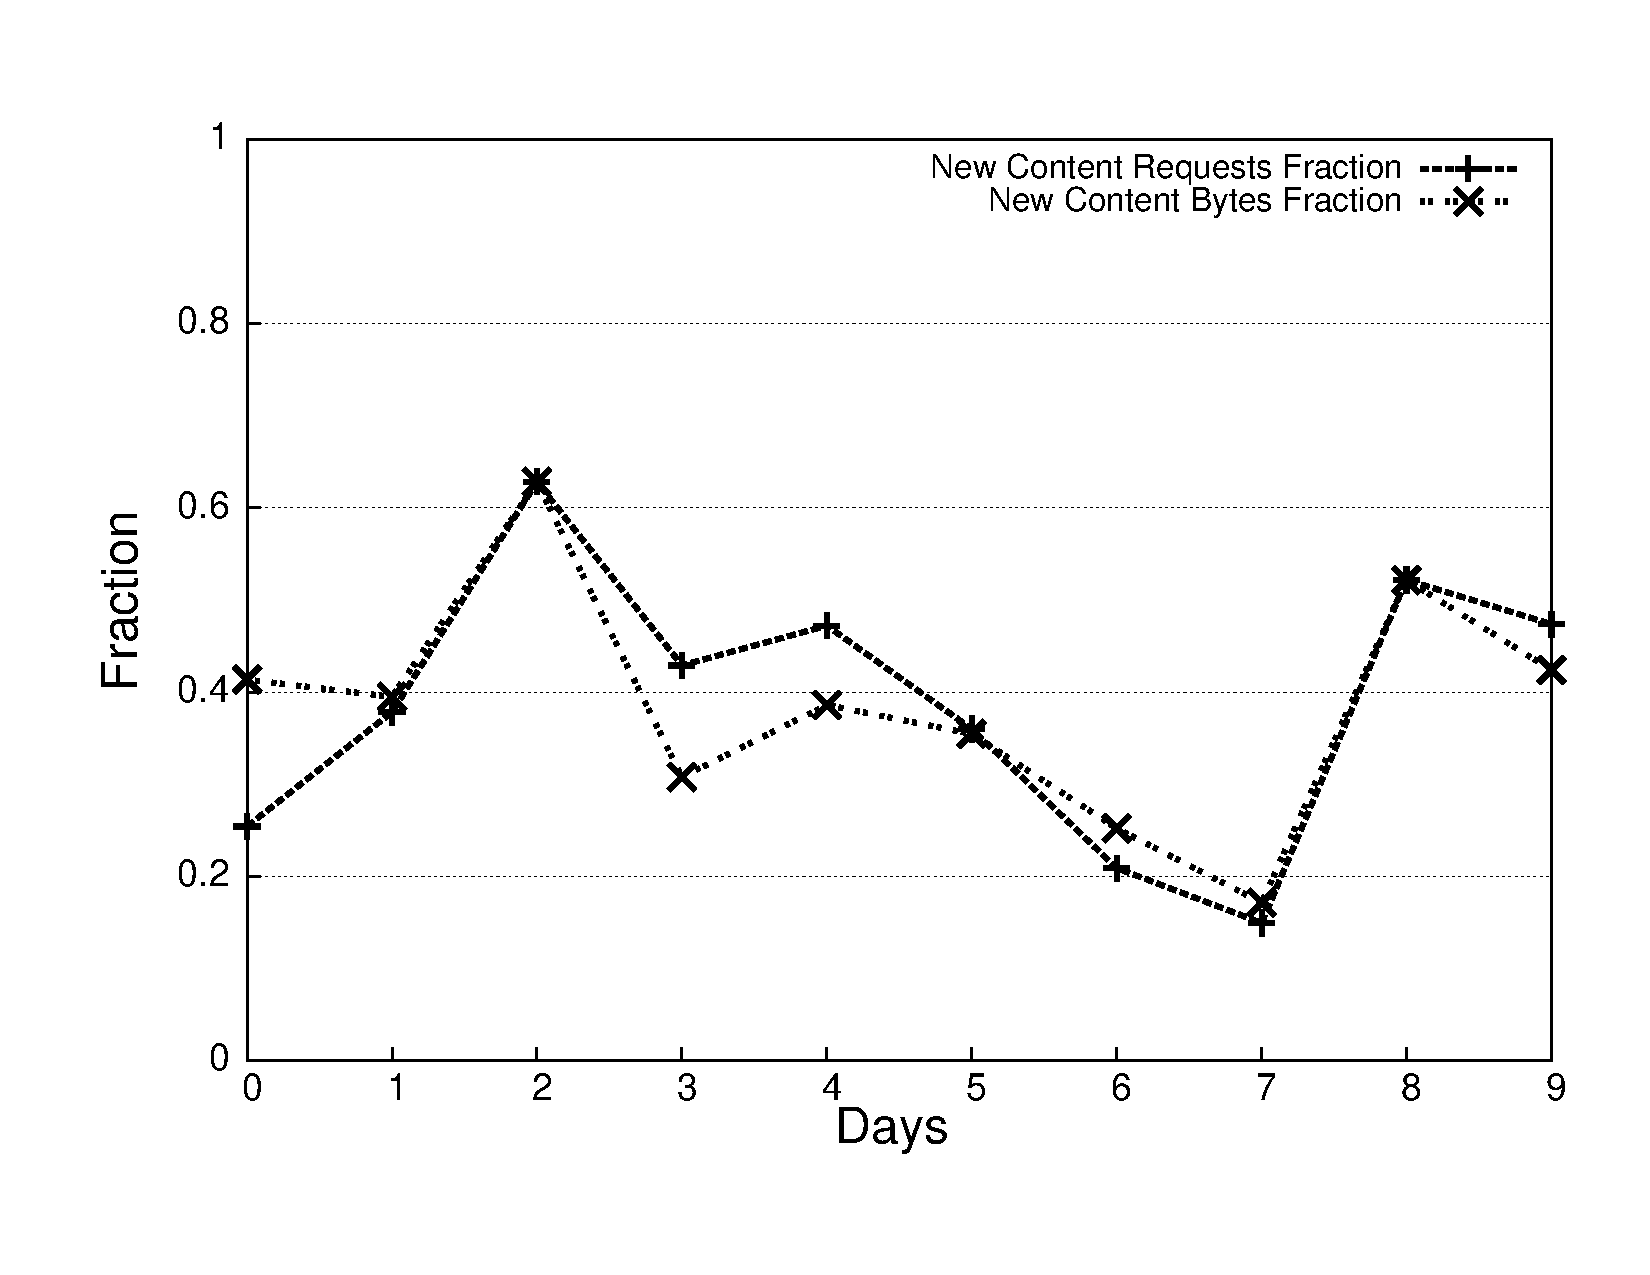
\includegraphics[scale=0.30]{graphSet1/shortvideos/churnNews.pdf}
%}
%\subfigure[MLU]{
%\vspace{2in}
%%	\includegraphics[scale=0.30]{graphSet1/shortvideos/mlunew.pdf}
%}
%\end{center}
%\caption{News videos trace. Since news  videos exhibit high churn on all days, performance of static placement schemes is consistently poor.}
%\label{fig:newsChurn}
%\end{figure*}



%\subsubsection{Entertainment Videos}







%\begin{figure*}	
%\begin{center}
%\subfigure[Churn Metric]{
%	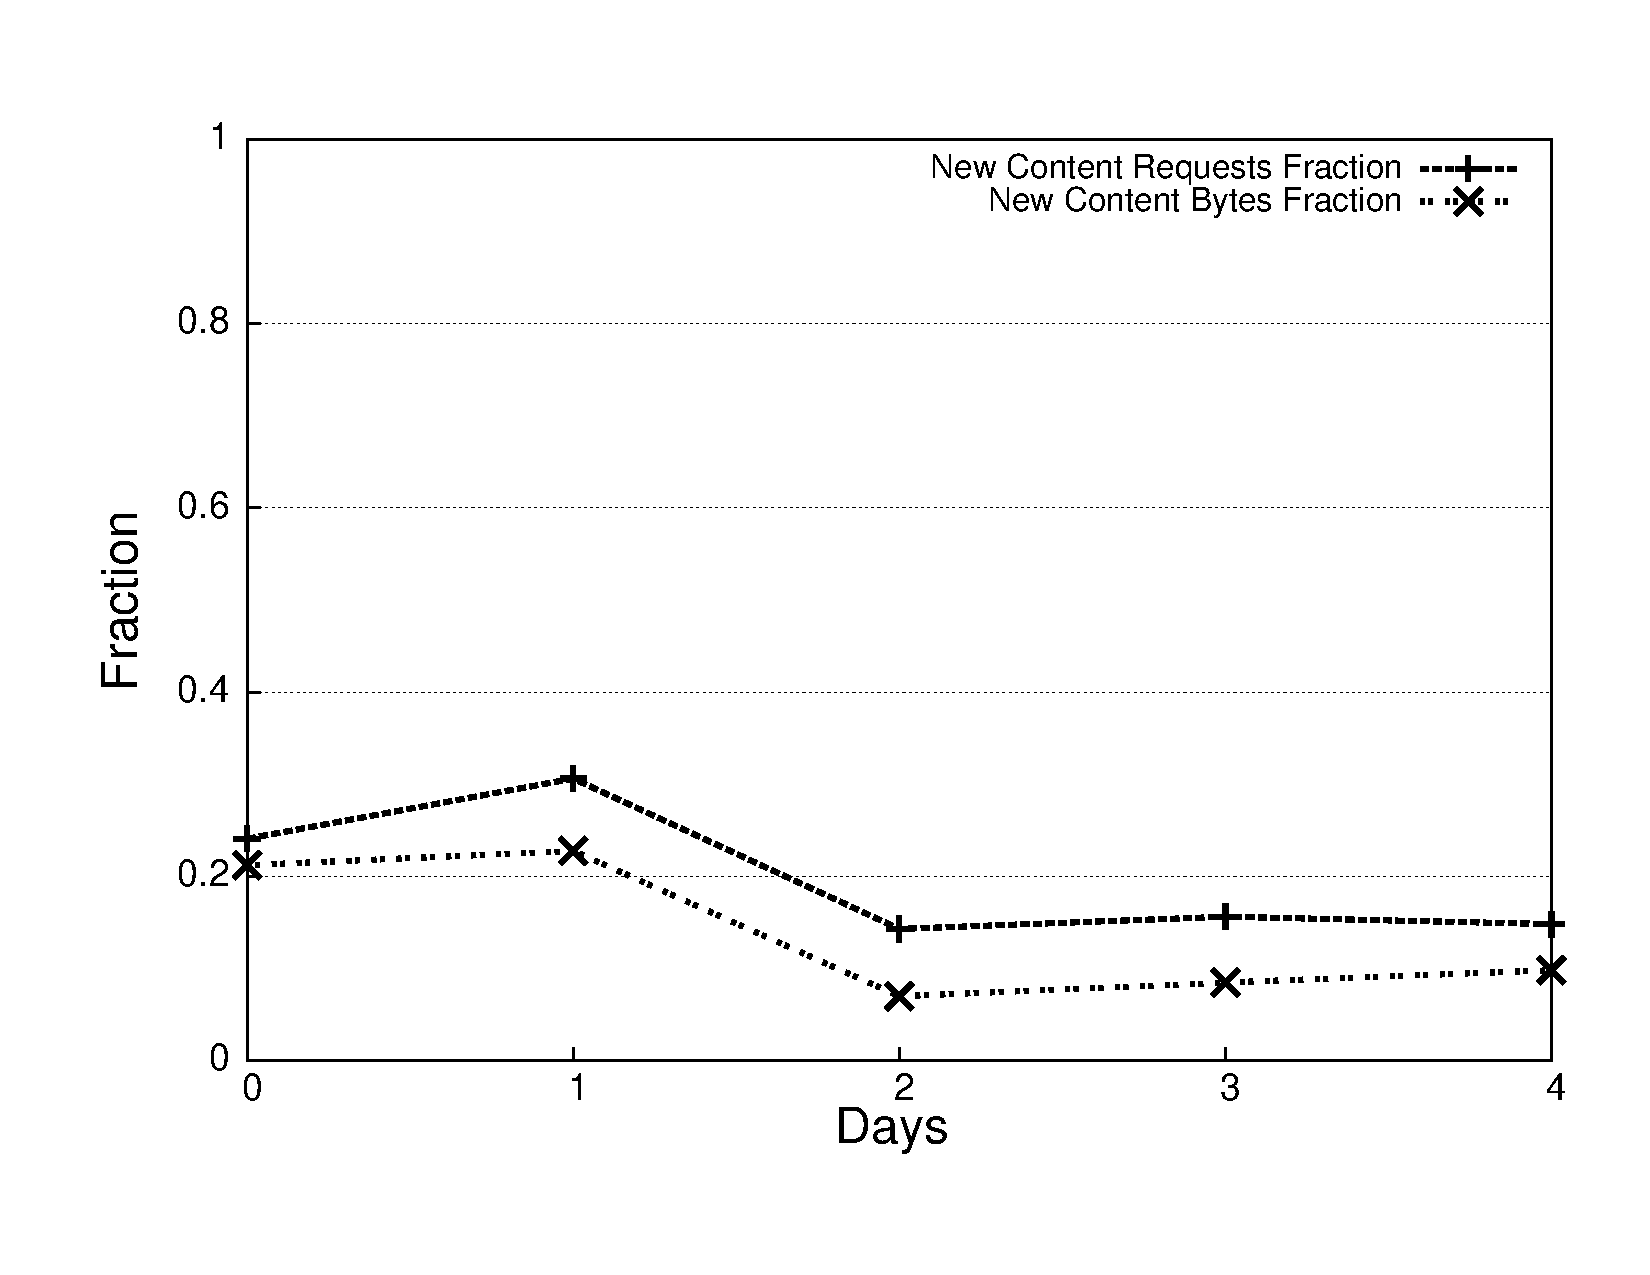
\includegraphics[scale=0.30]{graphSet1/tvAll/churnVideoAll.pdf}
%}
%\subfigure[MLU]{
%\vspace{2in}
%%	\includegraphics[scale=0.30]{graphSet1/shortvideos/mlunew.pdf}
%}
%\end{center}
%\caption{Entertainment videos combined trace. Churn metric and its correlation with the MLU for a static placement scheme.}
%\label{fig:entertainementChurn}
%\end{figure*}






%\begin{figure*}
%\begin{center}
%\subfigure[Abilene]{
%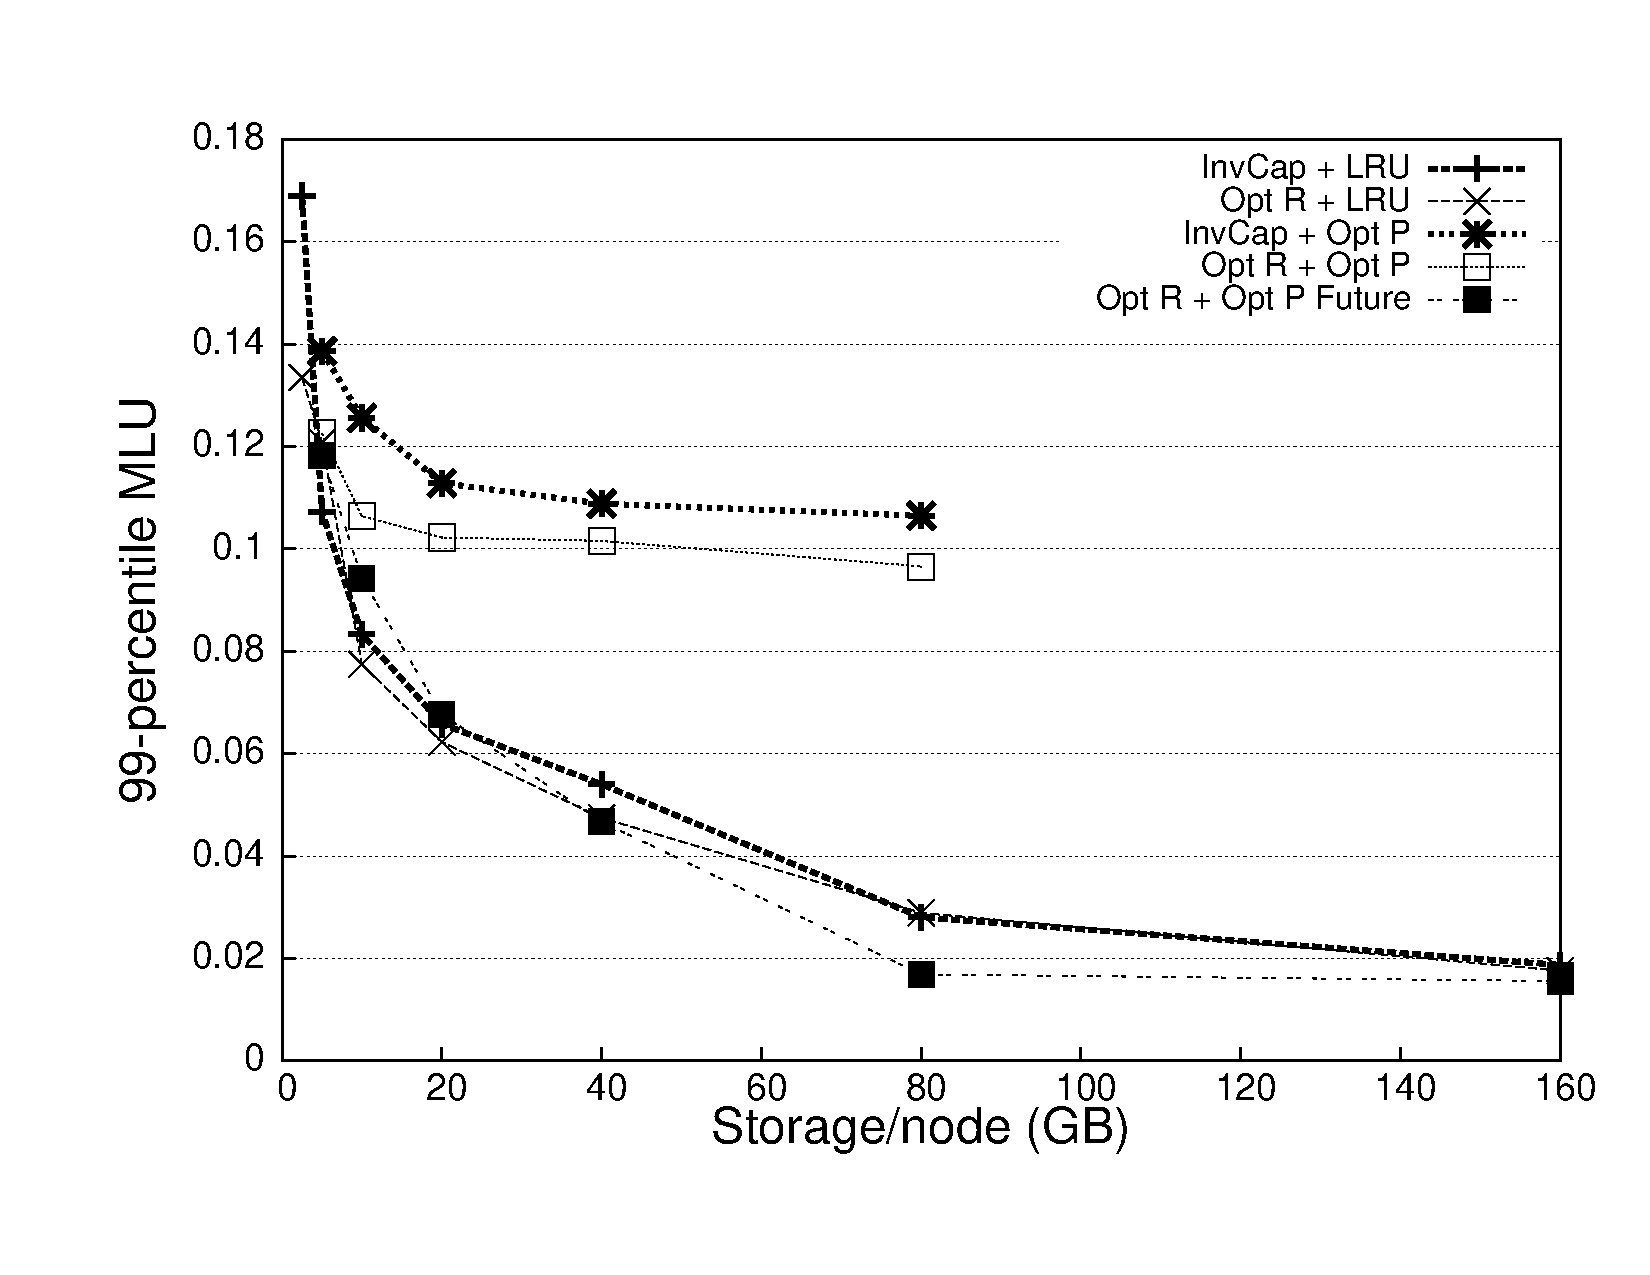
\includegraphics[scale=0.3]{graphSet1/longvideos/storageAbilene.pdf}
%}
%  \subfigure[ATT]{
%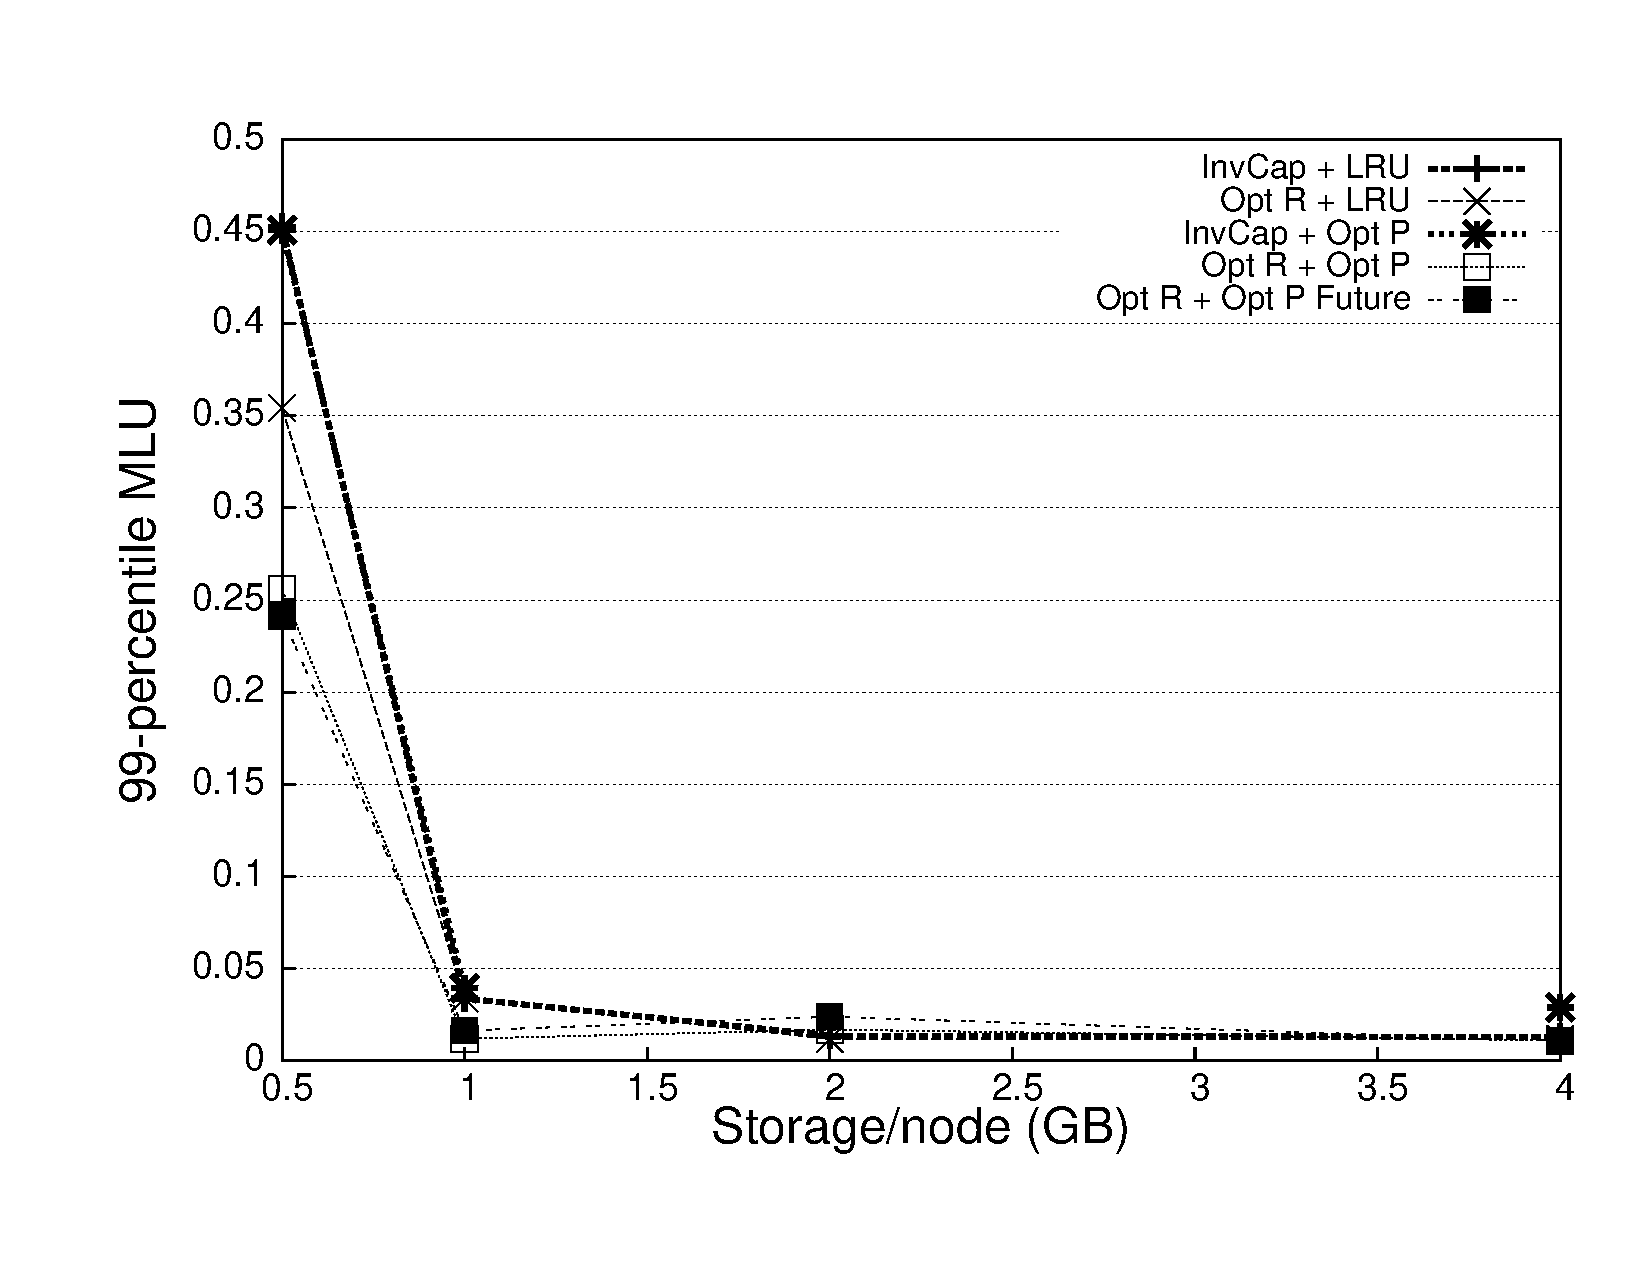
\includegraphics[scale=0.3]{graphSet1/longvideos/storageATT.pdf}
%}
%\end{center}
%\caption{TV shows trace 1(excluding  content smaller than 10 minutes.}
%\label{fig:longvideostrace}
%\end{figure*}



%\begin{figure*}
%\begin{center}
%\subfigure[Abilene]{
%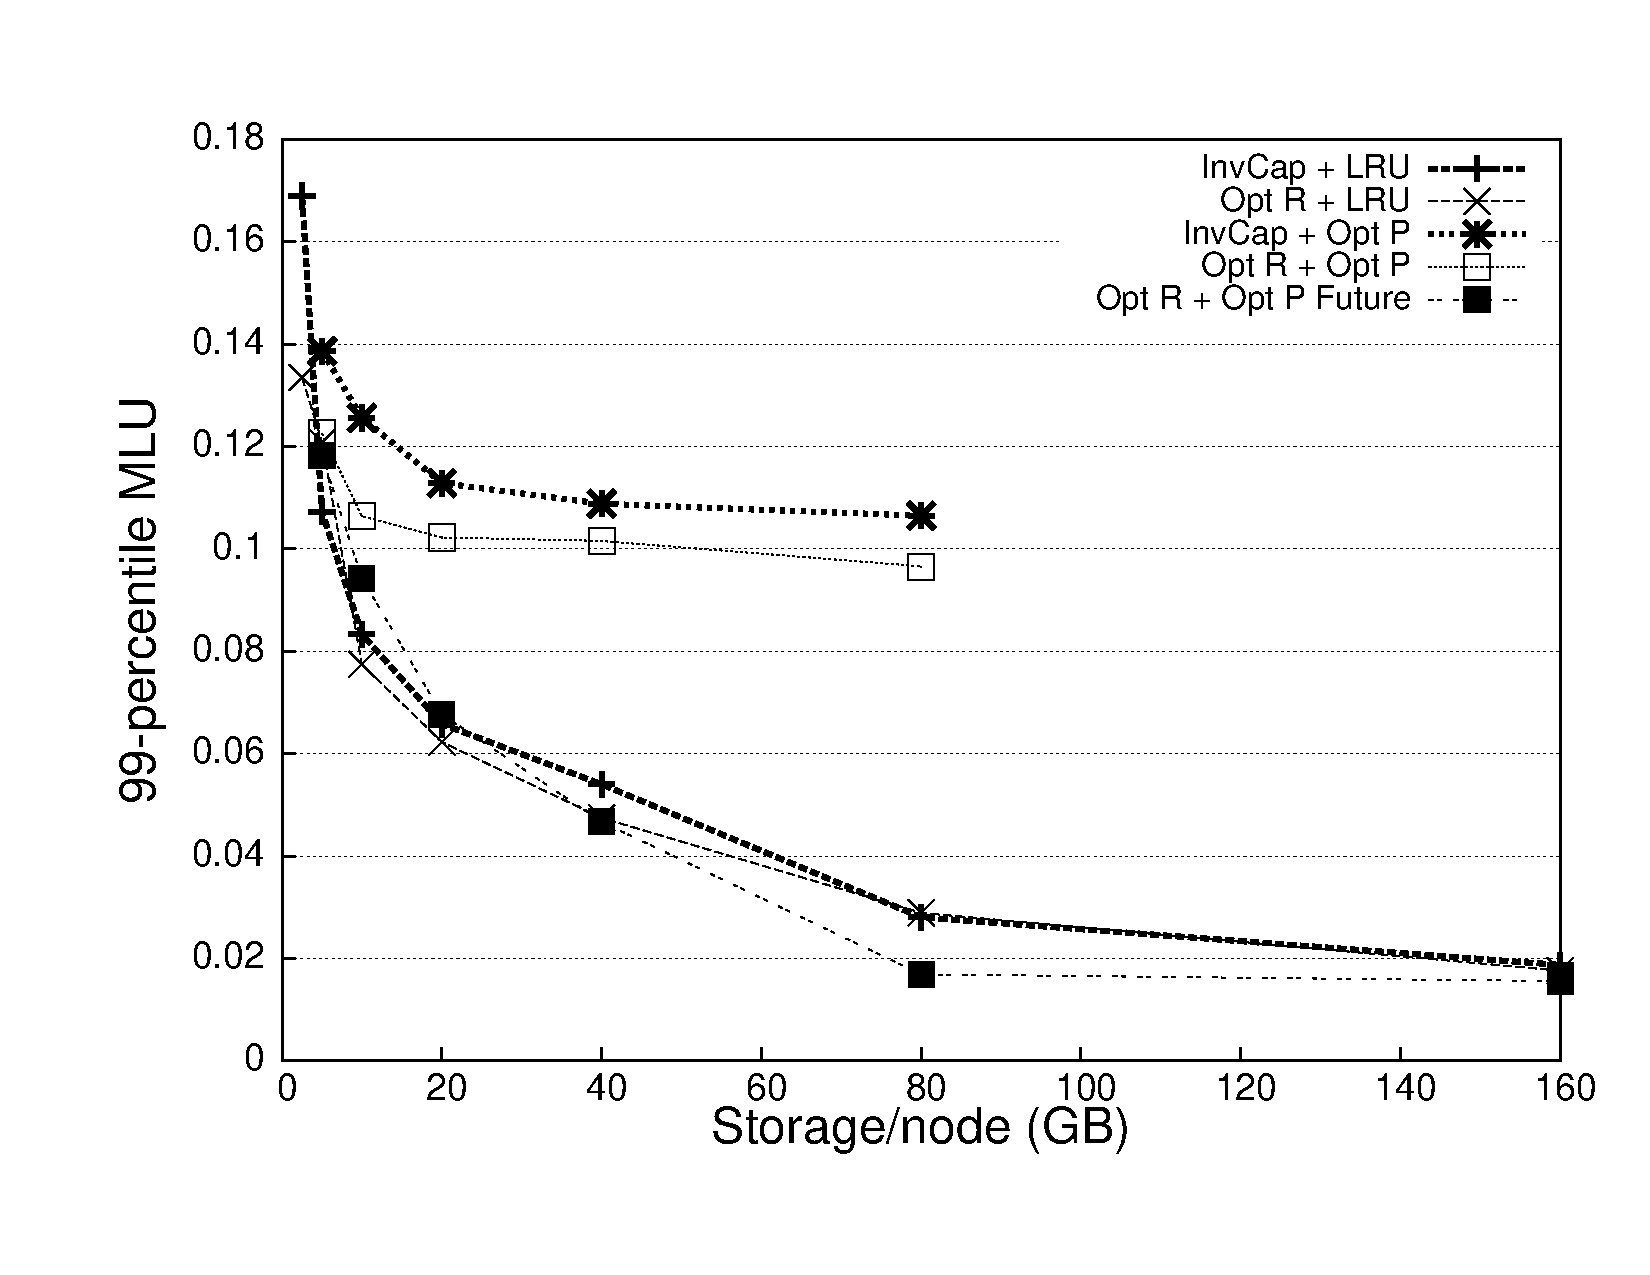
\includegraphics[scale=0.3]{graphSet1/longvideos/storageAbilene.pdf}
%}
%  \subfigure[ATT]{
%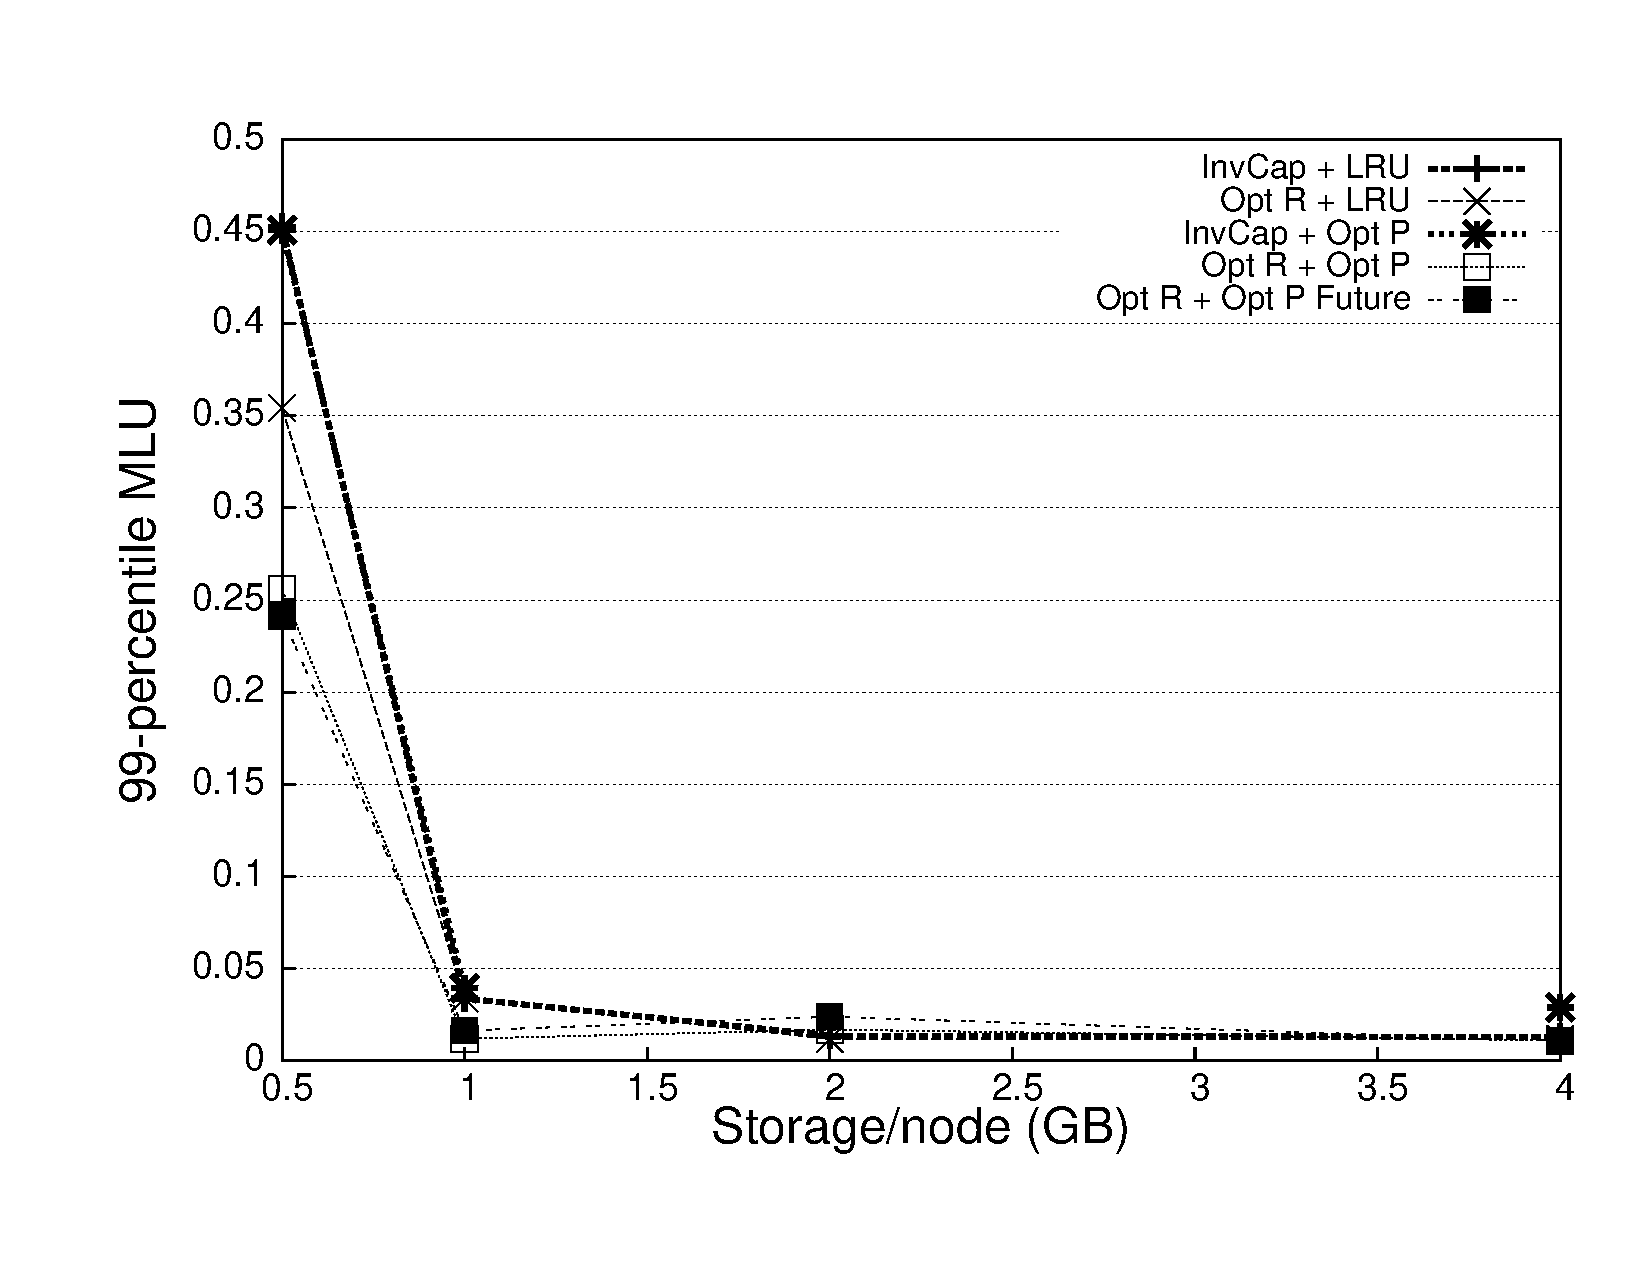
\includegraphics[scale=0.3]{graphSet1/longvideos/storageATT.pdf}
%}
%\end{center}
%\caption{TV shows trace 1(excluding  content smaller than 10 minutes.}
%\label{fig:longvideostrace}
%\end{figure*}





%\begin{figure*}
%\begin{center}
%\subfigure[Abilene]{
%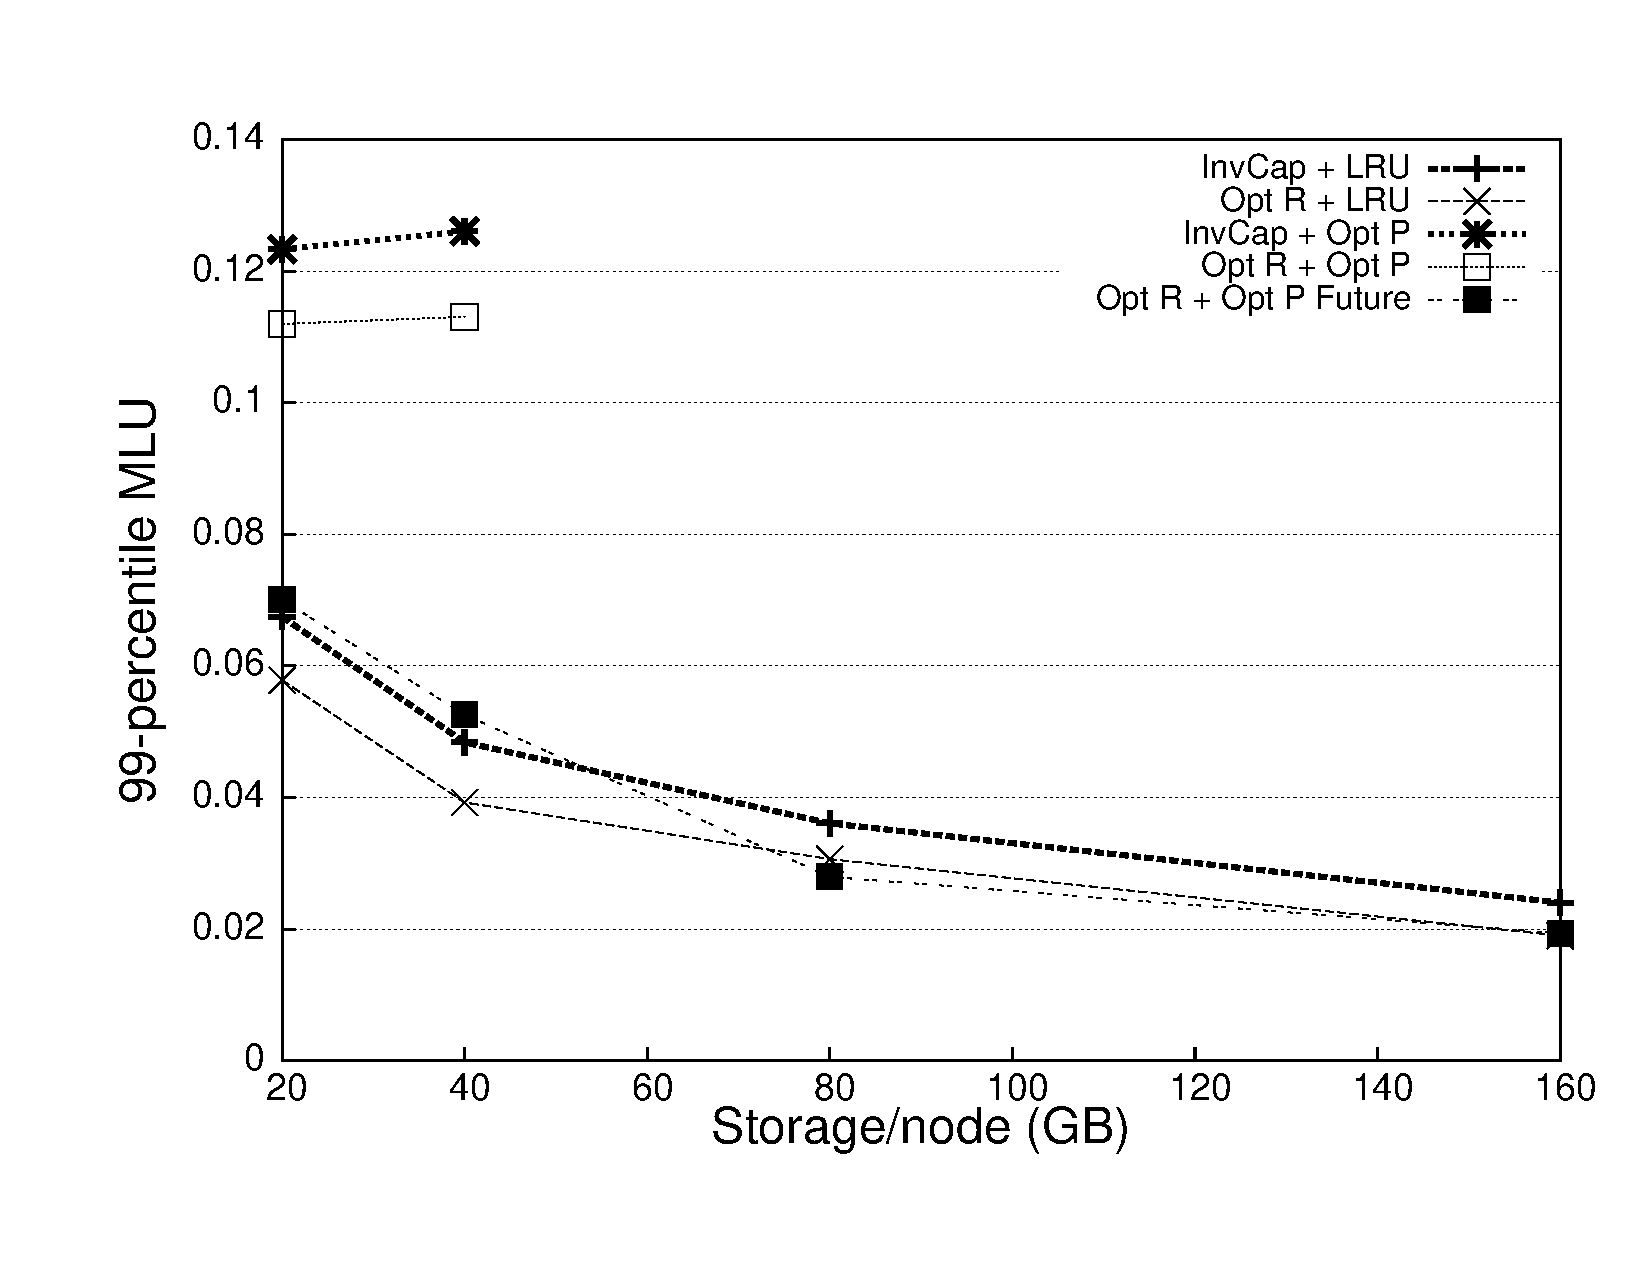
\includegraphics[scale=0.3]{graphSet1/tv1/AbileneTV1.pdf}
%}
%  \subfigure[ATT]{
%%\includegraphics[scale=0.3]{graphSet1/tv1/ATTTV1.pdf}
%}
%\end{center}
%\caption{TV shows trace 1.}
%\label{fig:longvideostrace}
%\end{figure*}




%\begin{figure*}
%\begin{center}
%\subfigure[Abilene]{
%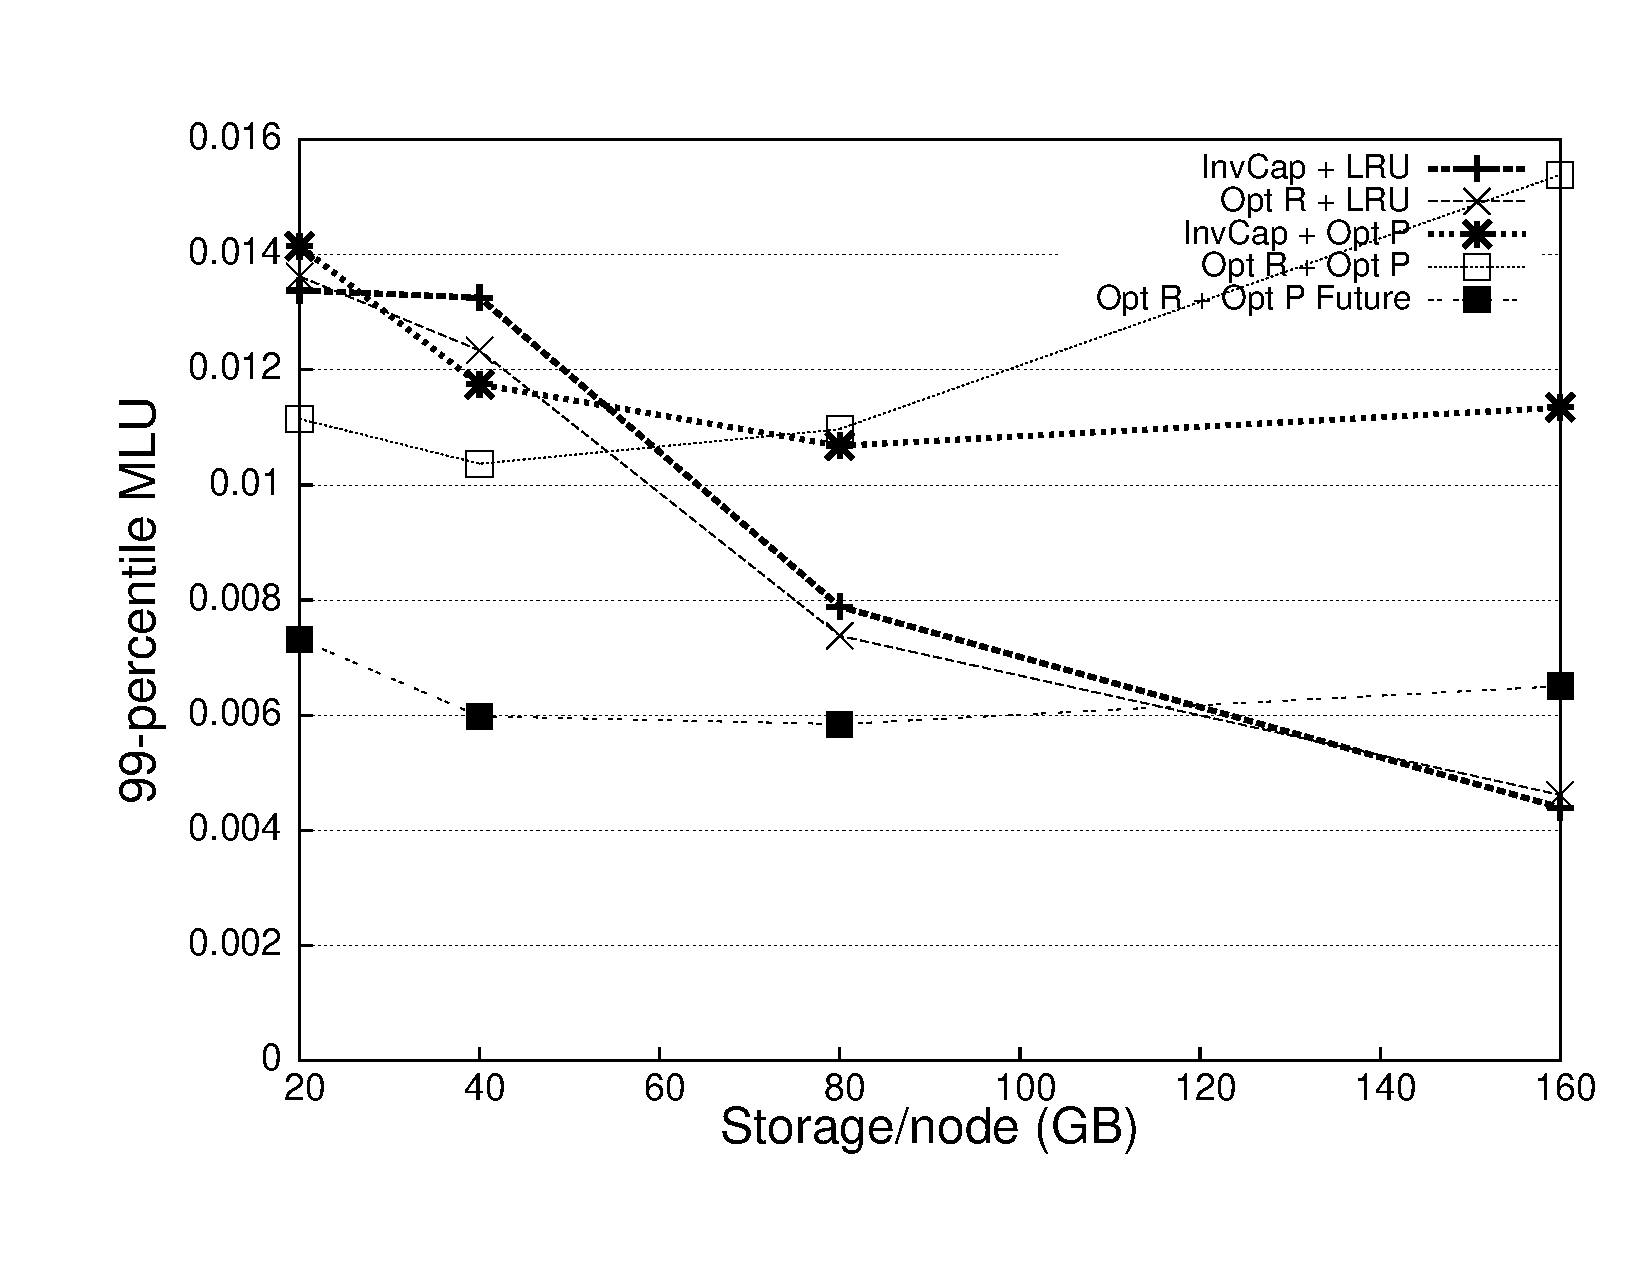
\includegraphics[scale=0.3]{graphSet1/tv2/AbileneTV2.pdf}
%}
%  \subfigure[ATT]{
%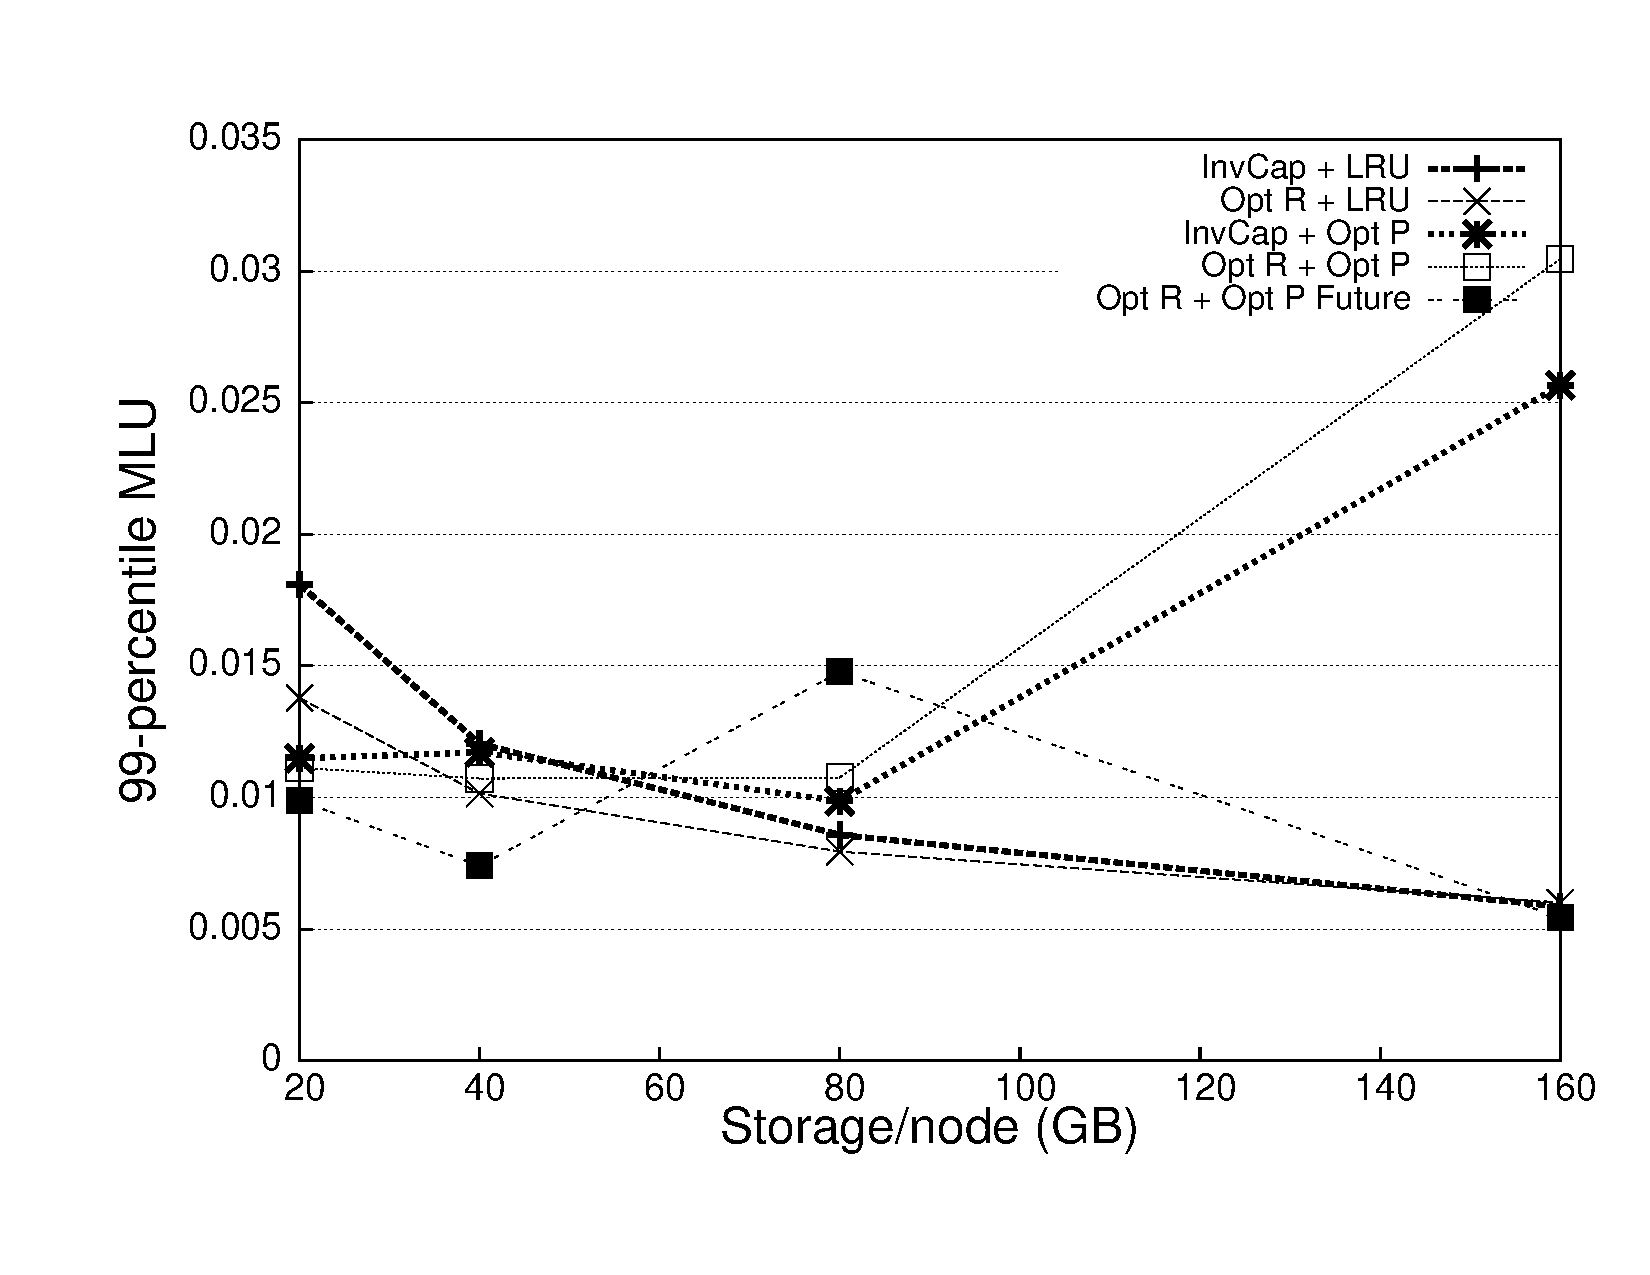
\includegraphics[scale=0.3]{graphSet1/tv2/ATTTV2.pdf}
%}
%\end{center}
%\caption{TV shows trace 2.}
%\label{fig:longvideostrace}
%\end{figure*}




%\begin{figure*}
%\begin{center}
%\subfigure[Abilene]{
%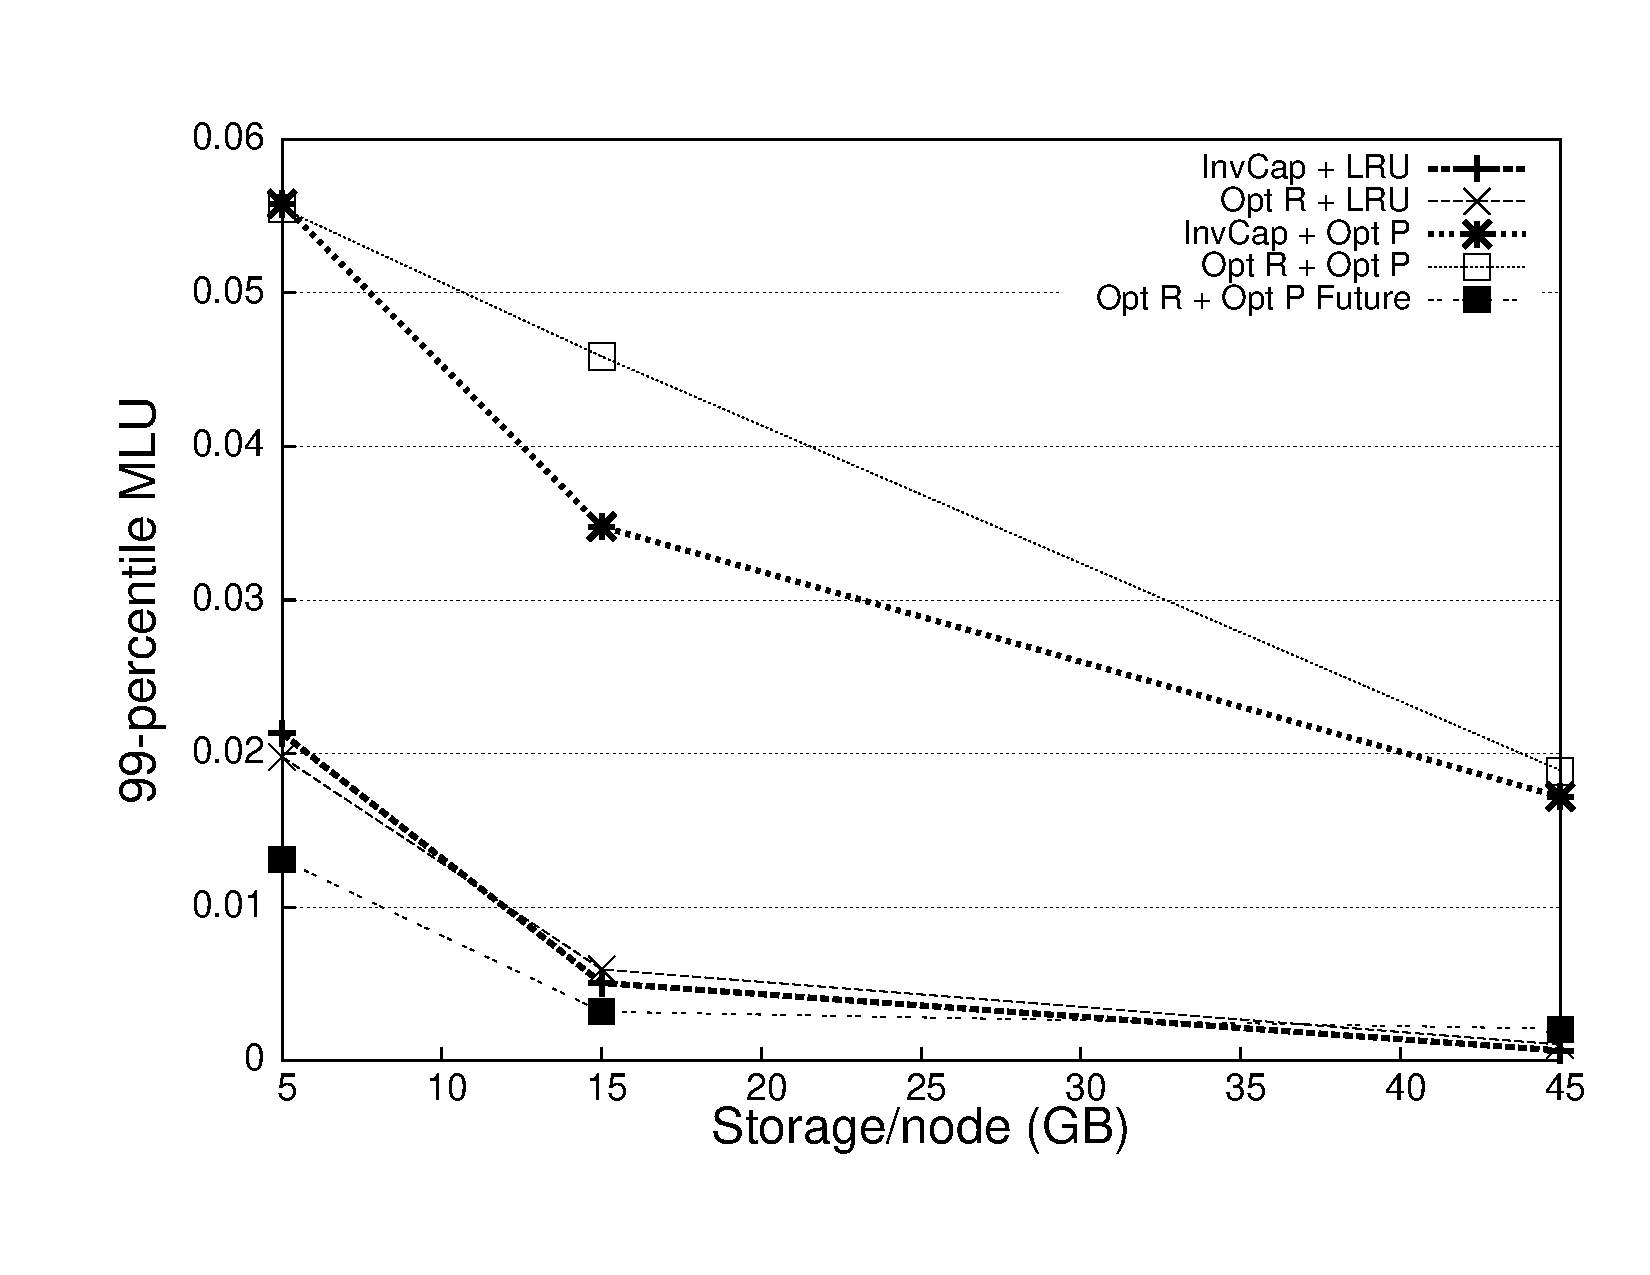
\includegraphics[scale=0.3]{graphSet1/tv3/AbileneTV3.pdf}
%}
%  \subfigure[ATT]{
%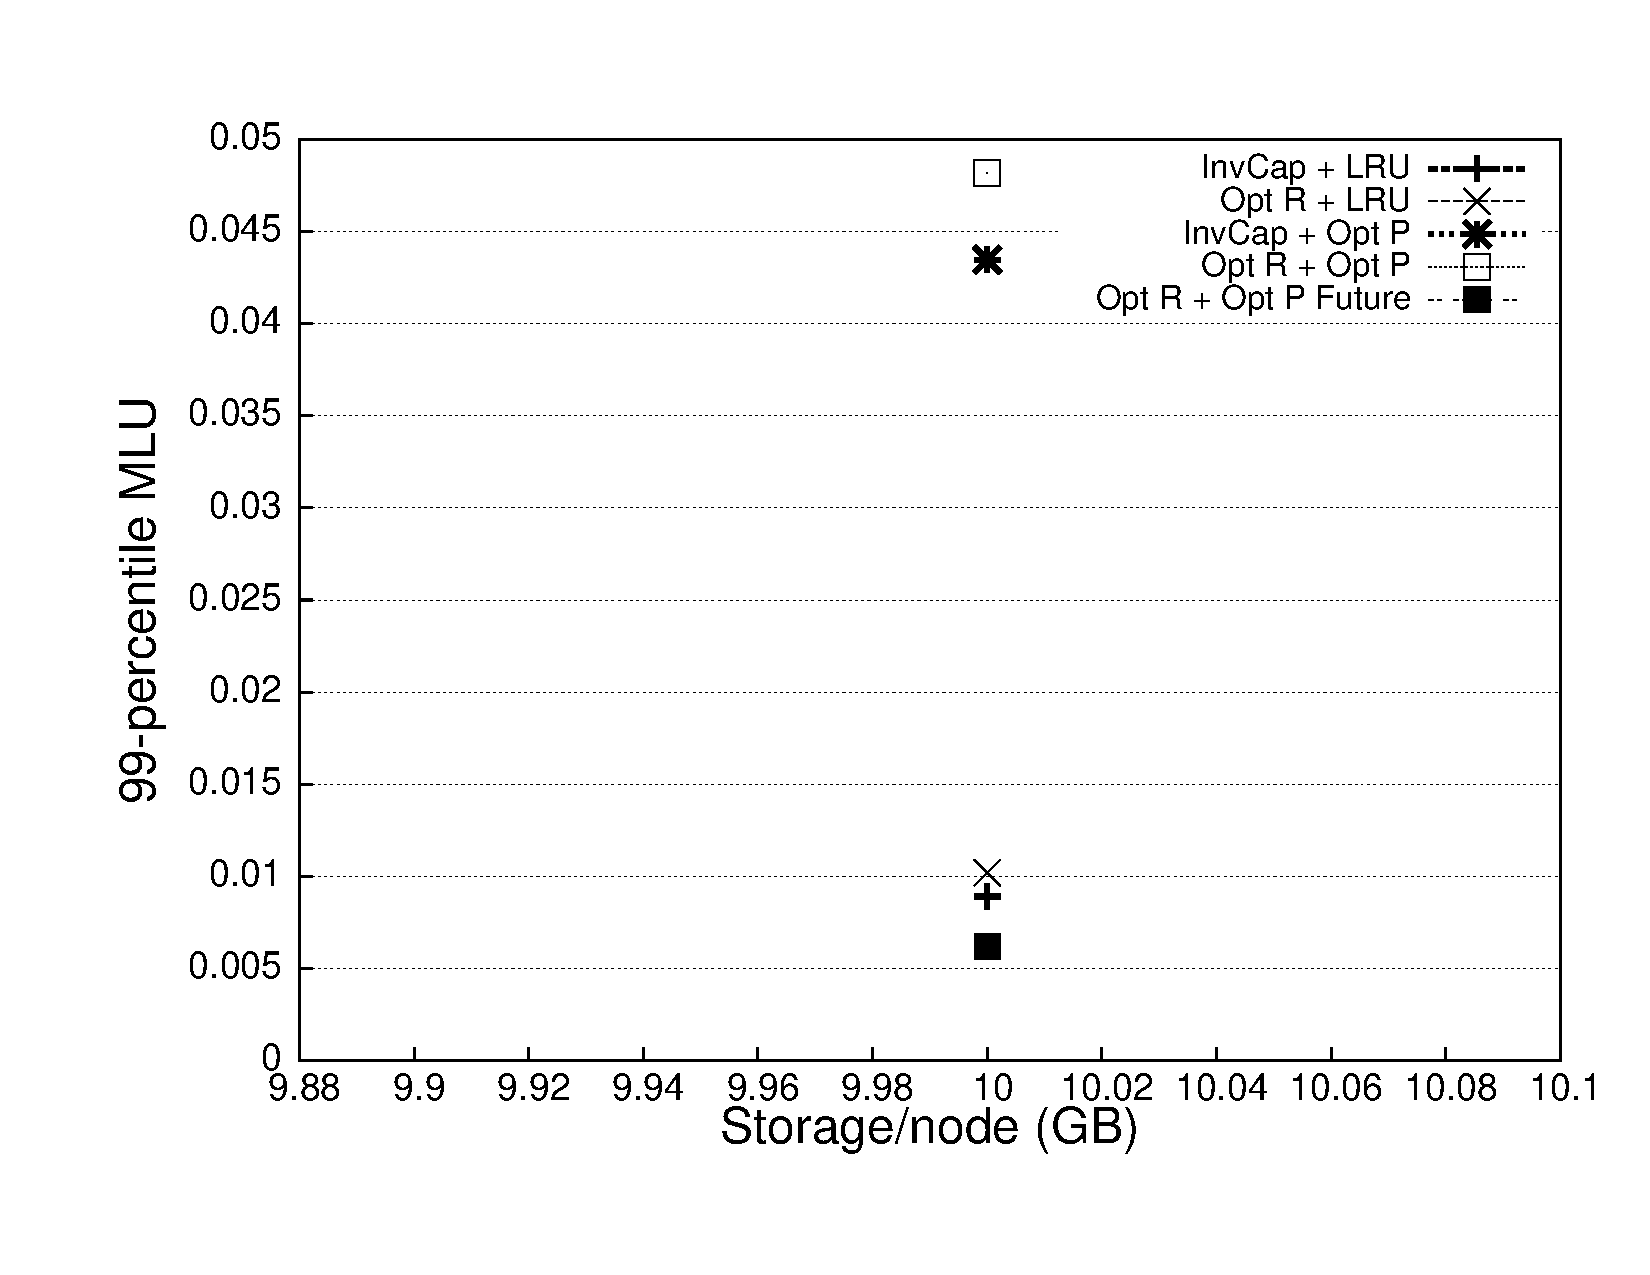
\includegraphics[scale=0.3]{graphSet1/tv3/ATTTV3.pdf}
%}
%\end{center}
%\caption{TV shows trace 3.}
%\label{fig:longvideostrace}
%\end{figure*}



%Long videos trace. Static placement schemes perform better than LRU Caching. Shows that the content popularity can be predicted based on based previous day's history. Compared  to InvCap + LRU, Opt R + Opt P performs 30\% better for Abilene and 25\% better for ATT topology.

%\begin{figure*}	
%\begin{center}
%\subfigure[Churn Metric]{
%	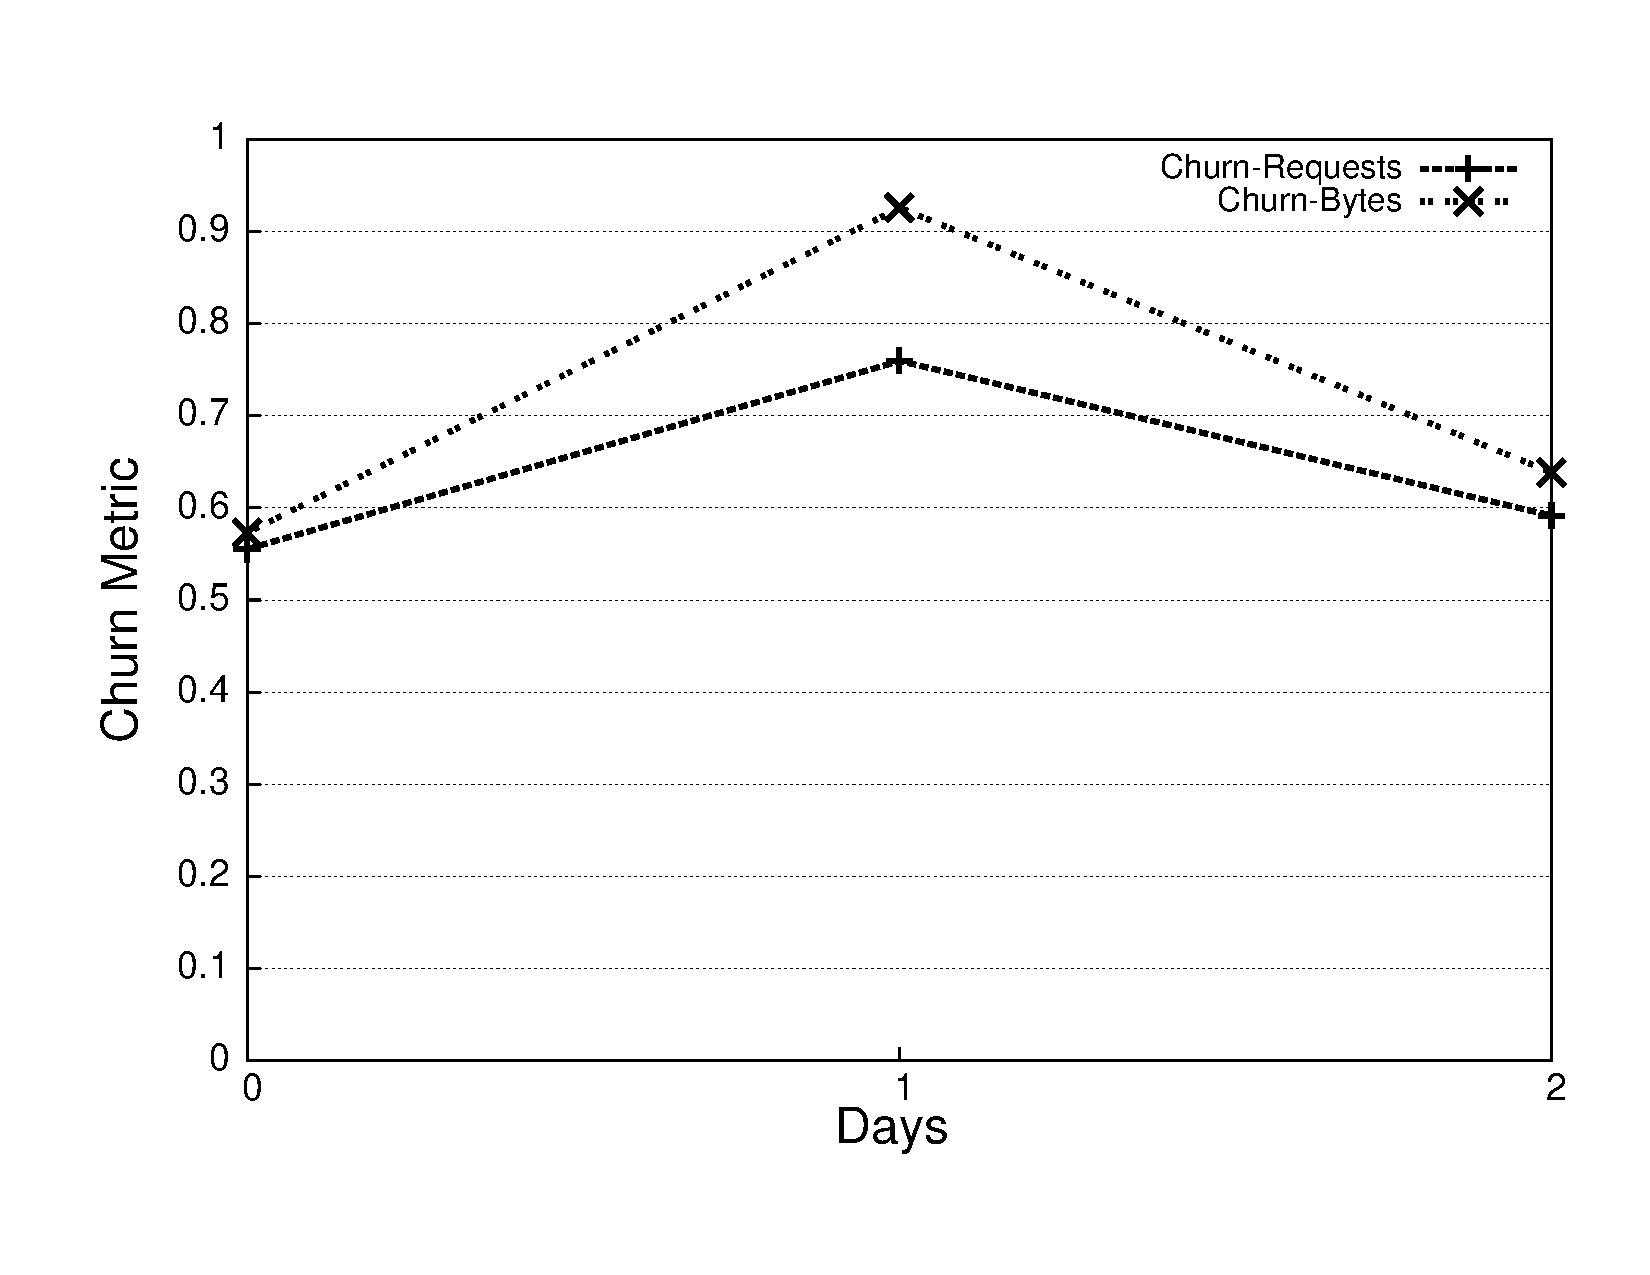
\includegraphics[scale=0.30]{graphSet1/longvideos/churnNewvideo1.pdf}
%}
%\subfigure[MLU]{
%\vspace{2in}
%%	\includegraphics[scale=0.30]{graphSet1/shortvideos/mlunew.pdf}
%}
%\end{center}
%\caption{TV shows trace. On the day 1 of the trace, churn is significantly higher due to which static placement performs poorly. }
%\label{fig:shortvideostatic}
%\end{figure*}


%\subsection{All On-Demand Videos Analysis}
%
%\begin{figure*}
%\begin{center}
%\subfigure[Abilene]{
%	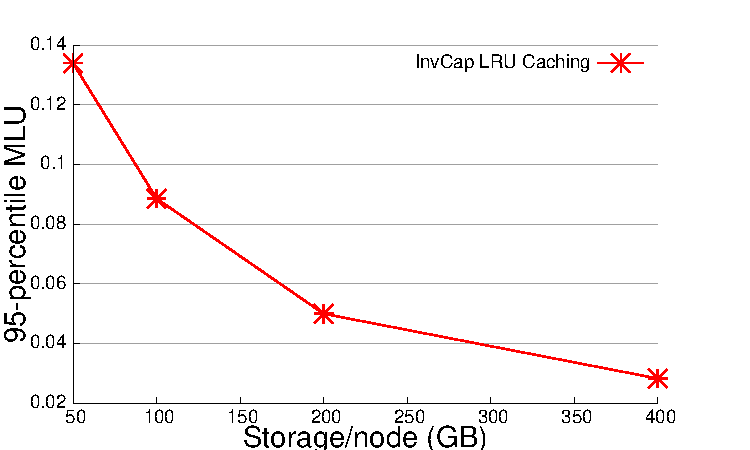
\includegraphics[scale=0.65]{graphSet1/onedayall/mlu_storage_AbileneAll.pdf}
%}
%\subfigure[Abilene]{
%	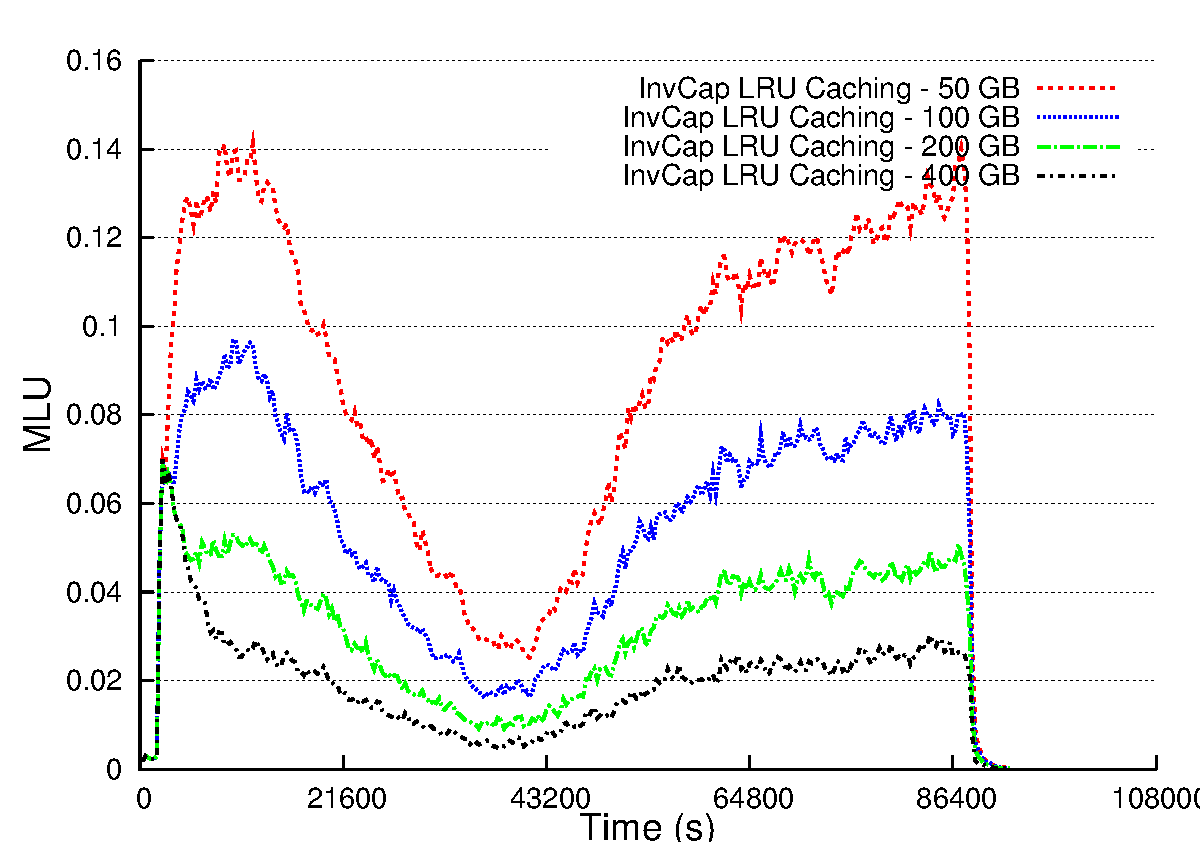
\includegraphics[scale=0.4]{graphSet1/onedayall/mlu_cachingAll.pdf}
%}
%\end{center}
%\caption{One Day Trace Of All On-Demand Videos.}
%\label{fig:allvideos}
%\end{figure*}










%\begin{figure*}
%\begin{center}
%\subfigure{
%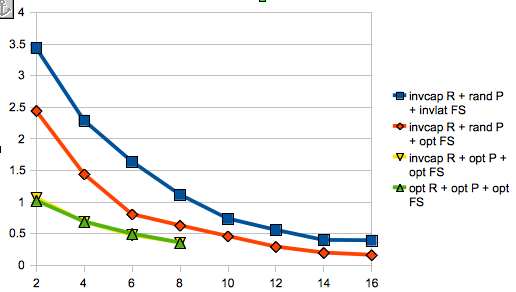
\includegraphics[scale=0.45]{graphSet1/att1.png}
%}
%  \subfigure{
%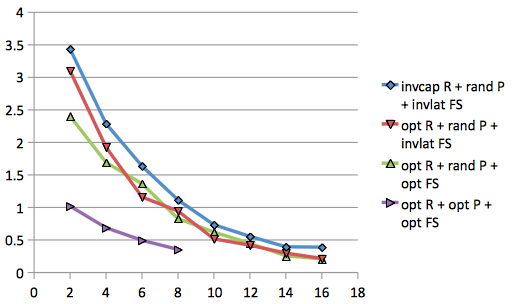
\includegraphics[scale=0.45]{graphSet1/att2.png}
%}
%\end{center}
%\caption{Comparison of static placement strategies for US-ISP dataset. Results. x-axis : Replication Factor,  y-axis: MLU}
%\end{figure*}
%
%  \begin{figure*}
%  \begin{center}
%  \subfigure{
%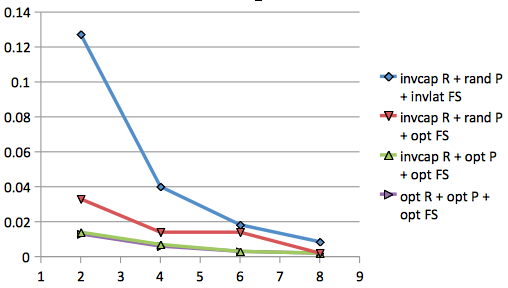
\includegraphics[scale=0.45]{graphSet1/abilene1.png}
%}
%  \subfigure{
%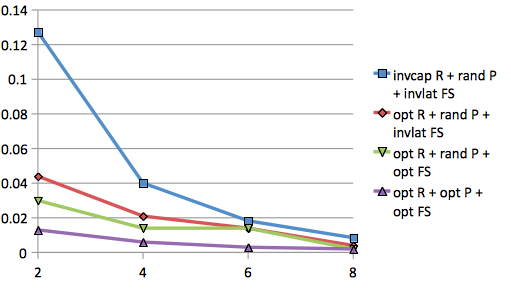
\includegraphics[scale=0.45]{graphSet1/abilene2.png}
%}
%\end{center}
%\caption{Comparison of static placement strategies for Abilene dataset. x-axis : Replication Factor,  y-axis: MLU}
%\end{figure*}



%
%
%
%  \begin{figure*}
%    \begin{center}
%  \subfigure[CDN]{
%  \vspace{2 in}
%}
%  \subfigure[US-ISP]{
%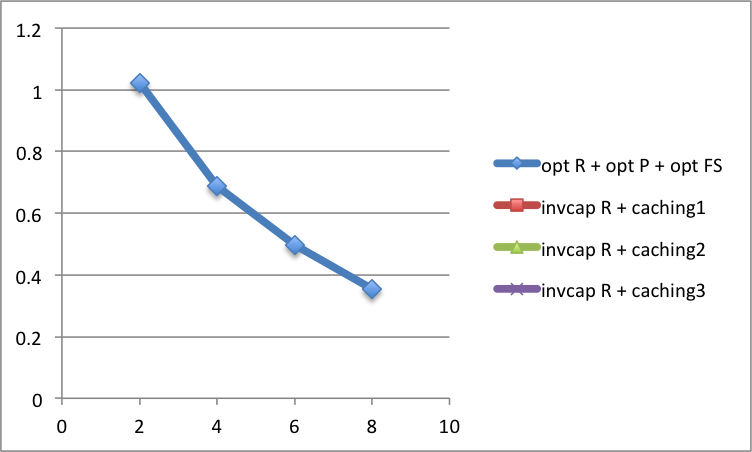
\includegraphics[scale=0.6]{graphSet1/attCaching.png}
%}
%  \subfigure[Abilene]{
%  \vspace{2 in}
%}
%\caption{Comparison of caching strategies against optimal placement strategy for CDN, US-ISP and Abilene traces.}
%    \end{center}
%\end{figure*}
%
%
%
%  \begin{figure*}
%    \begin{center}
%  \subfigure[CDN]{
%  \vspace{2 in}
%}
%  \subfigure[US-ISP]{
%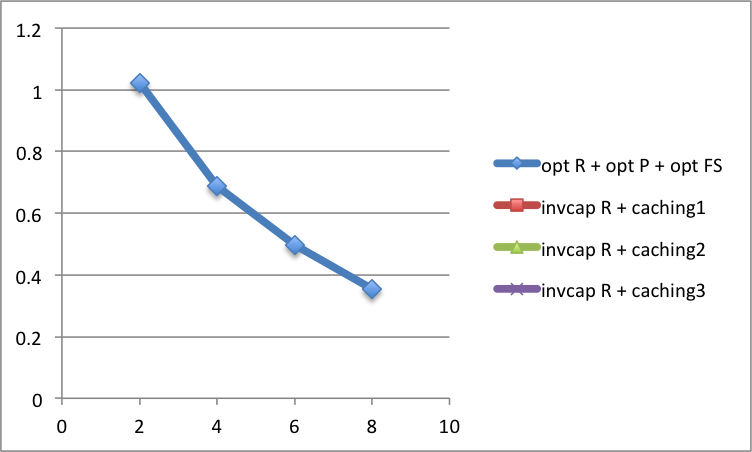
\includegraphics[scale=0.6]{graphSet1/attCaching.png}
%}
%  \subfigure[Abilene]{
%  \vspace{2 in}
%}
%\end{center}
%\caption{Frequency of content placement update.}
%\end{figure*}
%





%\subsection{Short Videos Trace}
%
%Q. Which placement scheme performs best ?
%A. Based on these results we find that a hybrid placement scheme which periodically updates its static placement performs best for short videos trace. 
%
%Q. Difference between invcap routing and optimal routing ?
%A. There is less than 10\% difference between optimal routing and InvCap routing but more than 20\% difference between optimal routing with next best placement scheme.
%
%
%%First, we compare the performance of static placement schemes. These schemes optimize one or more  of placement, flow split and the routing in the network. Our goal for this experiment is to understand that the contribution of optimizing each of  placement, routing and flow splits in reducing the network cost. For each experiment, we vary the replication factor and compare the network cost for all schemes.
%
%First, we compare the performance of static placement schemes. In Section 2, we had outlined the three classes of static placement schemes  - demand oblivious, heuristic, and optimal. Each placement scheme is combined with either a simple static shortest path strategy, i. e., InvCap or optimal routing strategy based on previously measured traffic demands. A combination of three placement and two routing schemes yields six possible TE schemes. 
%
%
%We find that static placement schemes suffer from the drawback of a significant fraction of requests going to origin server, which increases congestion at links near the PoP/s connected to the origin. There are two reasons for requests going to the origin server. First new content is published after the placement is computed. Second, requests for content which has not been accessed recently and is evicted from the network also go to the origin.
%Increasing the storage in the network does not solve this problem for new content. 
%
%
%
%But a purely static placement scheme is not practical because it causes a significant fraction of requests to go to the origin server. Such a scheme defeats the purpose of the content distribution service itself. And moreover it increases inter domain traffic for the ISP.
%



%\begin{figure*}
%\begin{center}
%\subfigure[Abilene]{
%	\includegraphics[scale=0.65]{graphSet1/shortvideos/mlu_storage_caching.pdf}
%}
%\subfigure[ATT]{
%	\includegraphics[scale=0.65]{graphSet1/shortvideos/mlu_storage_cachingATT.pdf}
%}
%\end{center}
%\caption{TE with dynamic placement (caching) for CDN short videos trace.}
%\label{fig:shortvideodynamic}
%\end{figure*}
%
%
%\begin{figure*}
%\begin{center}
%\subfigure[Abilene]{
%	\includegraphics[scale=0.65]{graphSet1/shortvideos/mlu_storage_hybrid.pdf}
%}
%\subfigure[ATT]{
%\vspace{2in}
%}
%\end{center}
%\caption{TE with hybrid (static + dynamic) placement for CDN short videos trace.}
%\label{fig:shortvideohybrid}
%\end{figure*}





%\begin{figure*}
%\begin{center}
%\includegraphics[scale=0.65]{graphSet1/longvideos/storageATTMovies.pdf}
%\end{center}
%\caption{Long videos trace on ATT topology. Opt R + Opt PR scheme (blue dot) is fairly close to Opt R + Opt PR  Future (green dot) }
%\label{fig:longvideostraceATT}
%\end{figure*}
%
%
%\begin{figure*}
%\begin{center}
%\includegraphics[scale=1]{graphSet1/longvideos/mlu.pdf}
%\end{center}
%\caption{Long Videos Trace, 100 GB/node, MLU timeline. This shows that we are getting a spike in MLU in going from 10 GB/node to 100 GB/node in Figure \ref{fig:longvideostrace} because update bandwidth during placement is very high.}
%\label{fig:mluovertimelongvideos100GB}
%\end{figure*}



% A caching algorithm determines  a content placement and flow splits, but not the routing in the network. We compare caching strategies against optimal placement and flow split strategy which uses InvCap routing. For all caching strategies, we use InvCap routing in the network. This ensures an even comparison between static placement and caching schemes. 


%
%\subsection{Long Videos Trace}
%
%
%
%\subsection{ISP Traffic Matrix Based Synthetic Traces}
%
%We compared seven traffic engineering schemes discussed in \ref{sec:TEscheme} for 10 randomly selected traffic matrices from Abilene and US-iSP datasets. For each traffic matrix, we performed two experiments: (1) All content is globally popular  (2) All content is  locally popular. In Figure 1 and Figure 2, we present the MLU of the network for each traffic engineering scheme for different levels of replication.
%
%Our comparison of  the four classes of traffic engineering schemes discussed in Section \ref{sec:TEscheme} reveals the following relative ordering among them: (Optimal Placement + Routing) = (Simple Routing + Optimal Placement)   $>$ 
%(Optimal Routing + Simple Placement) $>$ (Simple Routing + Simple Placement)
%
%Optimal Placement with a InvCap routing scheme (InvCapOptimalPlacement)  performs identical to the joint optimal solution of MLU and routing (OptimalPlacementRouting) in all the graphs. This shows that an ISP does not need to optimize both placement as well as routing; optimal routing has almost no utility if the placement can be optimized in the network. 
%
%% Explanation : 
%
%In contrast, optimal routing coupled with a simple placement strategy (random placement with InvCap Split OR random placement with InvLatency Split) performs is clearly a sub-optimal traffic engineering scheme. Comparing InvCapOptimalPlacement with InvCapRandomPlacementInvCapSplit or  InvCapRandomPlacementInvLatencySplit leads to the conclusion that optimizing  placement is more valuable for traffic engineering than optimizing routing in the network. Optimizing either placement or routing performs significantly better than not optimizing any of them as in the schemes InvCapRandomPlacementInvCapSplit  and InvCapRandomPlacementInvlatencySplit.
%
%For the content with local popularity, the difference between optimal placement scheme and other schemes is significantly higher. In US-ISP and Abilene topologies, optimal placement schemes have a MLU of less than 1/10th of other schemes for a replication factor of 2. This ratio of relative difference remains even for a higher replication factor say 4 and 6 (not visible in the graph).
%
%Optimizing flow splits plays an important role in computing optimal placement. Optimizing flow splits alone (InvCapRandomPlacementOptimalFlowSplits) helps diminish the difference between (simple routing + simple placement) schemes and InvCapOptimalPlacement (simple routing + optimal placement) scheme by as much as half in most cases. In the US-ISP topology,  optimizing only the flow splits performs better than optimizing routing in the network. It is true in the Abilene network in many cases when replication factor $> 4$.
%
%The marginal utility of additional replication replication decreases for all schemes. The convex nature of the curves in Figure 1 and Figure 2 shows that the MLU reduces by a smaller fraction with each additional replica of content.  Adding replica of a content reduces the network traffic due to that content since content can be served from a nearby node. With each additional replica, the fractional reduction in traffic is smaller and hence MLU reduces by a smaller amount.





%But, the relative difference between (Optimal Routing + Simple Placement) and (Simple Routing + Simple Placement) strategies decreases with increasing replication. This shows that replication benefits all schemes. 

%\textbf{ InvCap + Optimal Placement == Optimal:}InvCap+OptimalPlacement scheme performs the same as Optimal Routing + Placement scheme. 
%
%\textbf{InvCap + Optimal Routing $>=$ Optimal Routing + Simple Placement}
%
%\textbf{Where is InvCap + Random Placement + Optimal Flow Splits ?}
%
%\textbf{Global vs GlobalLocal:}
%
%Abilene : One Gravity + One Real TM : GlobalLocal + Global
%
%ATT : One Gravity + One Real TM : GlobalLocal + Global



%  \begin{figure}
%  \begin{center}
%\includegraphics[scale=0.65]{AbileneResults.png}
% \end{center}
%\caption{Abilene Results}
%  \begin{center}
%\includegraphics[scale=0.6]{Legend.png}
% \end{center}
% 
%  \caption{Legend for Figure 1 and Figure 2}
% \end{figure}
% 
%  \begin{figure}[h]
%  \begin{center}
%\includegraphics[scale=0.75]{AbileneLocal.png}
% \end{center}
%	  \caption{AbileneLocal}
% \end{figure}
%
% 
%  \begin{figure}[h]
%  \begin{center}
%\includegraphics[scale=0.75]{ATTGlobal.png}
% \end{center}
%	  \caption{ATTGlobal}
% \end{figure}
% 
%
%  \begin{figure}[h]
%  \begin{center}
%\includegraphics[scale=0.75]{ATTLocal.png}
% \end{center}
%	  \caption{ATTLocal}
% \end{figure}
 
%Sub points:
%
%	It holds for a small degree of replication
%	
%	It holds for multiple topologies
%	
%	It holds for multiple demand patterns
%	
%	It holds both with and without partial replication
